% Options for packages loaded elsewhere
\PassOptionsToPackage{unicode}{hyperref}
\PassOptionsToPackage{hyphens}{url}
\PassOptionsToPackage{dvipsnames,svgnames,x11names}{xcolor}
%
\documentclass[
]{article}
\usepackage{amsmath,amssymb}
\usepackage{iftex}
\ifPDFTeX
  \usepackage[T1]{fontenc}
  \usepackage[utf8]{inputenc}
  \usepackage{textcomp} % provide euro and other symbols
\else % if luatex or xetex
  \usepackage{unicode-math} % this also loads fontspec
  \defaultfontfeatures{Scale=MatchLowercase}
  \defaultfontfeatures[\rmfamily]{Ligatures=TeX,Scale=1}
\fi
\usepackage{lmodern}
\ifPDFTeX\else
  % xetex/luatex font selection
\fi
% Use upquote if available, for straight quotes in verbatim environments
\IfFileExists{upquote.sty}{\usepackage{upquote}}{}
\IfFileExists{microtype.sty}{% use microtype if available
  \usepackage[]{microtype}
  \UseMicrotypeSet[protrusion]{basicmath} % disable protrusion for tt fonts
}{}
\makeatletter
\@ifundefined{KOMAClassName}{% if non-KOMA class
  \IfFileExists{parskip.sty}{%
    \usepackage{parskip}
  }{% else
    \setlength{\parindent}{0pt}
    \setlength{\parskip}{6pt plus 2pt minus 1pt}}
}{% if KOMA class
  \KOMAoptions{parskip=half}}
\makeatother
\usepackage{xcolor}
\usepackage[margin=1in]{geometry}
\usepackage{color}
\usepackage{fancyvrb}
\newcommand{\VerbBar}{|}
\newcommand{\VERB}{\Verb[commandchars=\\\{\}]}
\DefineVerbatimEnvironment{Highlighting}{Verbatim}{commandchars=\\\{\}}
% Add ',fontsize=\small' for more characters per line
\usepackage{framed}
\definecolor{shadecolor}{RGB}{248,248,248}
\newenvironment{Shaded}{\begin{snugshade}}{\end{snugshade}}
\newcommand{\AlertTok}[1]{\textcolor[rgb]{0.94,0.16,0.16}{#1}}
\newcommand{\AnnotationTok}[1]{\textcolor[rgb]{0.56,0.35,0.01}{\textbf{\textit{#1}}}}
\newcommand{\AttributeTok}[1]{\textcolor[rgb]{0.13,0.29,0.53}{#1}}
\newcommand{\BaseNTok}[1]{\textcolor[rgb]{0.00,0.00,0.81}{#1}}
\newcommand{\BuiltInTok}[1]{#1}
\newcommand{\CharTok}[1]{\textcolor[rgb]{0.31,0.60,0.02}{#1}}
\newcommand{\CommentTok}[1]{\textcolor[rgb]{0.56,0.35,0.01}{\textit{#1}}}
\newcommand{\CommentVarTok}[1]{\textcolor[rgb]{0.56,0.35,0.01}{\textbf{\textit{#1}}}}
\newcommand{\ConstantTok}[1]{\textcolor[rgb]{0.56,0.35,0.01}{#1}}
\newcommand{\ControlFlowTok}[1]{\textcolor[rgb]{0.13,0.29,0.53}{\textbf{#1}}}
\newcommand{\DataTypeTok}[1]{\textcolor[rgb]{0.13,0.29,0.53}{#1}}
\newcommand{\DecValTok}[1]{\textcolor[rgb]{0.00,0.00,0.81}{#1}}
\newcommand{\DocumentationTok}[1]{\textcolor[rgb]{0.56,0.35,0.01}{\textbf{\textit{#1}}}}
\newcommand{\ErrorTok}[1]{\textcolor[rgb]{0.64,0.00,0.00}{\textbf{#1}}}
\newcommand{\ExtensionTok}[1]{#1}
\newcommand{\FloatTok}[1]{\textcolor[rgb]{0.00,0.00,0.81}{#1}}
\newcommand{\FunctionTok}[1]{\textcolor[rgb]{0.13,0.29,0.53}{\textbf{#1}}}
\newcommand{\ImportTok}[1]{#1}
\newcommand{\InformationTok}[1]{\textcolor[rgb]{0.56,0.35,0.01}{\textbf{\textit{#1}}}}
\newcommand{\KeywordTok}[1]{\textcolor[rgb]{0.13,0.29,0.53}{\textbf{#1}}}
\newcommand{\NormalTok}[1]{#1}
\newcommand{\OperatorTok}[1]{\textcolor[rgb]{0.81,0.36,0.00}{\textbf{#1}}}
\newcommand{\OtherTok}[1]{\textcolor[rgb]{0.56,0.35,0.01}{#1}}
\newcommand{\PreprocessorTok}[1]{\textcolor[rgb]{0.56,0.35,0.01}{\textit{#1}}}
\newcommand{\RegionMarkerTok}[1]{#1}
\newcommand{\SpecialCharTok}[1]{\textcolor[rgb]{0.81,0.36,0.00}{\textbf{#1}}}
\newcommand{\SpecialStringTok}[1]{\textcolor[rgb]{0.31,0.60,0.02}{#1}}
\newcommand{\StringTok}[1]{\textcolor[rgb]{0.31,0.60,0.02}{#1}}
\newcommand{\VariableTok}[1]{\textcolor[rgb]{0.00,0.00,0.00}{#1}}
\newcommand{\VerbatimStringTok}[1]{\textcolor[rgb]{0.31,0.60,0.02}{#1}}
\newcommand{\WarningTok}[1]{\textcolor[rgb]{0.56,0.35,0.01}{\textbf{\textit{#1}}}}
\usepackage{longtable,booktabs,array}
\usepackage{calc} % for calculating minipage widths
% Correct order of tables after \paragraph or \subparagraph
\usepackage{etoolbox}
\makeatletter
\patchcmd\longtable{\par}{\if@noskipsec\mbox{}\fi\par}{}{}
\makeatother
% Allow footnotes in longtable head/foot
\IfFileExists{footnotehyper.sty}{\usepackage{footnotehyper}}{\usepackage{footnote}}
\makesavenoteenv{longtable}
\usepackage{graphicx}
\makeatletter
\def\maxwidth{\ifdim\Gin@nat@width>\linewidth\linewidth\else\Gin@nat@width\fi}
\def\maxheight{\ifdim\Gin@nat@height>\textheight\textheight\else\Gin@nat@height\fi}
\makeatother
% Scale images if necessary, so that they will not overflow the page
% margins by default, and it is still possible to overwrite the defaults
% using explicit options in \includegraphics[width, height, ...]{}
\setkeys{Gin}{width=\maxwidth,height=\maxheight,keepaspectratio}
% Set default figure placement to htbp
\makeatletter
\def\fps@figure{htbp}
\makeatother
\setlength{\emergencystretch}{3em} % prevent overfull lines
\providecommand{\tightlist}{%
  \setlength{\itemsep}{0pt}\setlength{\parskip}{0pt}}
\setcounter{secnumdepth}{-\maxdimen} % remove section numbering
\newlength{\cslhangindent}
\setlength{\cslhangindent}{1.5em}
\newlength{\csllabelwidth}
\setlength{\csllabelwidth}{3em}
\newlength{\cslentryspacingunit} % times entry-spacing
\setlength{\cslentryspacingunit}{\parskip}
\newenvironment{CSLReferences}[2] % #1 hanging-ident, #2 entry spacing
 {% don't indent paragraphs
  \setlength{\parindent}{0pt}
  % turn on hanging indent if param 1 is 1
  \ifodd #1
  \let\oldpar\par
  \def\par{\hangindent=\cslhangindent\oldpar}
  \fi
  % set entry spacing
  \setlength{\parskip}{#2\cslentryspacingunit}
 }%
 {}
\usepackage{calc}
\newcommand{\CSLBlock}[1]{#1\hfill\break}
\newcommand{\CSLLeftMargin}[1]{\parbox[t]{\csllabelwidth}{#1}}
\newcommand{\CSLRightInline}[1]{\parbox[t]{\linewidth - \csllabelwidth}{#1}\break}
\newcommand{\CSLIndent}[1]{\hspace{\cslhangindent}#1}
\usepackage{fancyhdr}
\pagestyle{fancy}
\fancyhf{}
\lfoot[\thepage]{}
\rfoot[]{\thepage}
\fontsize{12}{22}
\selectfont
\usepackage{booktabs}
\usepackage{longtable}
\usepackage{array}
\usepackage{multirow}
\usepackage{wrapfig}
\usepackage{float}
\usepackage{colortbl}
\usepackage{pdflscape}
\usepackage{tabu}
\usepackage{threeparttable}
\usepackage{threeparttablex}
\usepackage[normalem]{ulem}
\usepackage{makecell}
\usepackage{xcolor}
\ifLuaTeX
  \usepackage{selnolig}  % disable illegal ligatures
\fi
\IfFileExists{bookmark.sty}{\usepackage{bookmark}}{\usepackage{hyperref}}
\IfFileExists{xurl.sty}{\usepackage{xurl}}{} % add URL line breaks if available
\urlstyle{same}
\hypersetup{
  colorlinks=true,
  linkcolor={blue},
  filecolor={Maroon},
  citecolor={Blue},
  urlcolor={Blue},
  pdfcreator={LaTeX via pandoc}}

\title{
\includegraphics[width=10cm,height=\textheight]{IEO-logo2.png}}
\author{}
\date{\vspace{-2.5em}}

\begin{document}
\maketitle


\pagenumbering{gobble}

%\begin{titlepage}
\begin{flushleft}
\Large{\textbf{SAR Metodología}}\\
\vspace*{2\baselineskip}
\LARGE{\textbf{Implementación metodológica SAR en pesquería de chirla \textit{Chamelea galllina} en el Golfo de Cádiz, España}}\\
\vspace*{5\baselineskip}
\Large{Grupo de Trabajo FEMP 04}\\
\vspace*{1\baselineskip}
\Large{Instituto Español de Oceanografía, Cádiz }\\
\vspace*{4\baselineskip}
\end{flushleft}
\begin{flushright}
\large{\textit{Mauricio Mardones}}\\
\large{\textit{Ana Magro}}\\
\vspace*{1\baselineskip}
\normalsize{\textbf{Fecha}}\\
Abril, 2024
\end{flushright}

% \end{titlepage}


\hypersetup{linkcolor = black}
\newpage
\pagenumbering{roman}
%\tableofcontents
%\addcontentsline{toc}{section}{\contentsname}

\newpage



\pagenumbering{arabic}
\hypersetup{linkcolor = blue}

{
\hypersetup{linkcolor=}
\setcounter{tocdepth}{3}
\tableofcontents
}
\newpage

\begin{Shaded}
\begin{Highlighting}[]
\FunctionTok{library}\NormalTok{(tidyverse)}
\FunctionTok{library}\NormalTok{(ggridges)}
\FunctionTok{library}\NormalTok{(readxl)}
\FunctionTok{library}\NormalTok{(here)}
\FunctionTok{library}\NormalTok{(lubridate)}
\FunctionTok{library}\NormalTok{(readr)}
\FunctionTok{library}\NormalTok{(ggthemes)}
\FunctionTok{library}\NormalTok{(hrbrthemes)}
\FunctionTok{library}\NormalTok{(kableExtra)}
\FunctionTok{library}\NormalTok{(gtsummary)}
\FunctionTok{library}\NormalTok{(egg)}
\FunctionTok{library}\NormalTok{(ggthemes)}
\FunctionTok{library}\NormalTok{(geosphere)}
\FunctionTok{library}\NormalTok{(sp)}
\FunctionTok{library}\NormalTok{(sf)}
\end{Highlighting}
\end{Shaded}

\hypertarget{contexto}{%
\section{CONTEXTO}\label{contexto}}

\hypertarget{data}{%
\section{DATA}\label{data}}

Existen tres tipos de archivos que contienen los datos de fauna y registros. Entre ellos, lo comun es la Columna \texttt{Estación} . Los archivos son \texttt{Datos\_estaciones\_ACUVEN\_3D\_IN-BENTO.xlsx}, \texttt{Fauna\_danos\_all.xlsx} y \texttt{Station.xlsx}

El archivo \texttt{Station.xlsx} tieme el area asociada
(\protect\hyperlink{ref-Indicator}{Indicator, n.d.})

\begin{Shaded}
\begin{Highlighting}[]
\NormalTok{fauna }\OtherTok{\textless{}{-}} \FunctionTok{read\_excel}\NormalTok{(}\FunctionTok{here}\NormalTok{(}\StringTok{"DATOS"}\NormalTok{,}
                         \StringTok{"Fauna\_danos\_all.xlsx"}\NormalTok{))}
\NormalTok{station }\OtherTok{\textless{}{-}} \FunctionTok{read\_excel}\NormalTok{(}\FunctionTok{here}\NormalTok{(}\StringTok{"DATOS"}\NormalTok{,}
                         \StringTok{"Station.xlsx"}\NormalTok{))}
\NormalTok{rendi }\OtherTok{\textless{}{-}} \FunctionTok{read\_excel}\NormalTok{(}\FunctionTok{here}\NormalTok{(}\StringTok{"DATOS"}\NormalTok{,}
                         \StringTok{"Datos\_estaciones\_ACUVEN\_3D\_IN{-}BENTO.xlsx"}\NormalTok{),}
                         \AttributeTok{skip =} \DecValTok{3}\NormalTok{)}
\end{Highlighting}
\end{Shaded}

\hypertarget{datos-fauna}{%
\subsection{Datos Fauna}\label{datos-fauna}}

\begin{Shaded}
\begin{Highlighting}[]
\FunctionTok{unique}\NormalTok{(fauna}\SpecialCharTok{$}\NormalTok{ID\_FINAL)}
\FunctionTok{names}\NormalTok{(fauna)}
\end{Highlighting}
\end{Shaded}

Agrupar por diversas variables

\begin{Shaded}
\begin{Highlighting}[]
\NormalTok{cantes }\OtherTok{\textless{}{-}}\NormalTok{ fauna }\SpecialCharTok{\%\textgreater{}\%} 
  \FunctionTok{group\_by}\NormalTok{(ID\_FINAL) }\SpecialCharTok{\%\textgreater{}\%}
  \FunctionTok{summarize}\NormalTok{(}\AttributeTok{SUM =} \FunctionTok{sum}\NormalTok{(}\StringTok{\textasciigrave{}}\AttributeTok{Total Indiv...49}\StringTok{\textasciigrave{}}\NormalTok{,}
                                     \AttributeTok{na.rm =} \ConstantTok{TRUE}\NormalTok{),}
            \AttributeTok{SUMPES =} \FunctionTok{sum}\NormalTok{(}\StringTok{\textasciigrave{}}\AttributeTok{Peso total (g)...50}\StringTok{\textasciigrave{}}\NormalTok{))}

\NormalTok{indsum }\OtherTok{\textless{}{-}} \FunctionTok{ggplot}\NormalTok{(cantes }\SpecialCharTok{\%\textgreater{}\%} 
                   \FunctionTok{drop\_na}\NormalTok{(ID\_FINAL))}\SpecialCharTok{+}
  \FunctionTok{geom\_col}\NormalTok{(}\FunctionTok{aes}\NormalTok{(}\AttributeTok{x =}\NormalTok{ID\_FINAL, }\AttributeTok{y=}\NormalTok{ SUM, }\AttributeTok{fill=}\NormalTok{ID\_FINAL))}\SpecialCharTok{+}
  \FunctionTok{theme\_few}\NormalTok{()}\SpecialCharTok{+}
  \FunctionTok{theme}\NormalTok{(}\AttributeTok{axis.text.x =} \FunctionTok{element\_text}\NormalTok{(}\AttributeTok{angle =} \DecValTok{90}\NormalTok{,}
                                     \AttributeTok{hjust =} \DecValTok{1}\NormalTok{,}
                                     \AttributeTok{vjust =} \FloatTok{0.5}\NormalTok{,}
                                     \AttributeTok{size =} \DecValTok{8}\NormalTok{),}
        \AttributeTok{legend.position =} \StringTok{"none"}\NormalTok{)}
  

\NormalTok{pessum }\OtherTok{\textless{}{-}} \FunctionTok{ggplot}\NormalTok{(cantes }\SpecialCharTok{\%\textgreater{}\%} 
                   \FunctionTok{drop\_na}\NormalTok{(ID\_FINAL))}\SpecialCharTok{+}
  \FunctionTok{geom\_col}\NormalTok{(}\FunctionTok{aes}\NormalTok{(}\AttributeTok{x =}\NormalTok{ID\_FINAL, }\AttributeTok{y=}\NormalTok{ SUMPES, }\AttributeTok{fill=}\NormalTok{ID\_FINAL))}\SpecialCharTok{+}
  \FunctionTok{theme\_few}\NormalTok{()}\SpecialCharTok{+}
  \FunctionTok{theme}\NormalTok{(}\AttributeTok{axis.text.x =} \FunctionTok{element\_text}\NormalTok{(}\AttributeTok{angle =} \DecValTok{90}\NormalTok{,}
                                     \AttributeTok{hjust =} \DecValTok{1}\NormalTok{,}
                                     \AttributeTok{vjust =} \FloatTok{0.5}\NormalTok{,}
                                     \AttributeTok{size =} \DecValTok{5}\NormalTok{),}
        \AttributeTok{legend.position =} \StringTok{"none"}\NormalTok{)}
\end{Highlighting}
\end{Shaded}

\begin{Shaded}
\begin{Highlighting}[]
\NormalTok{indsum}
\end{Highlighting}
\end{Shaded}

\begin{center}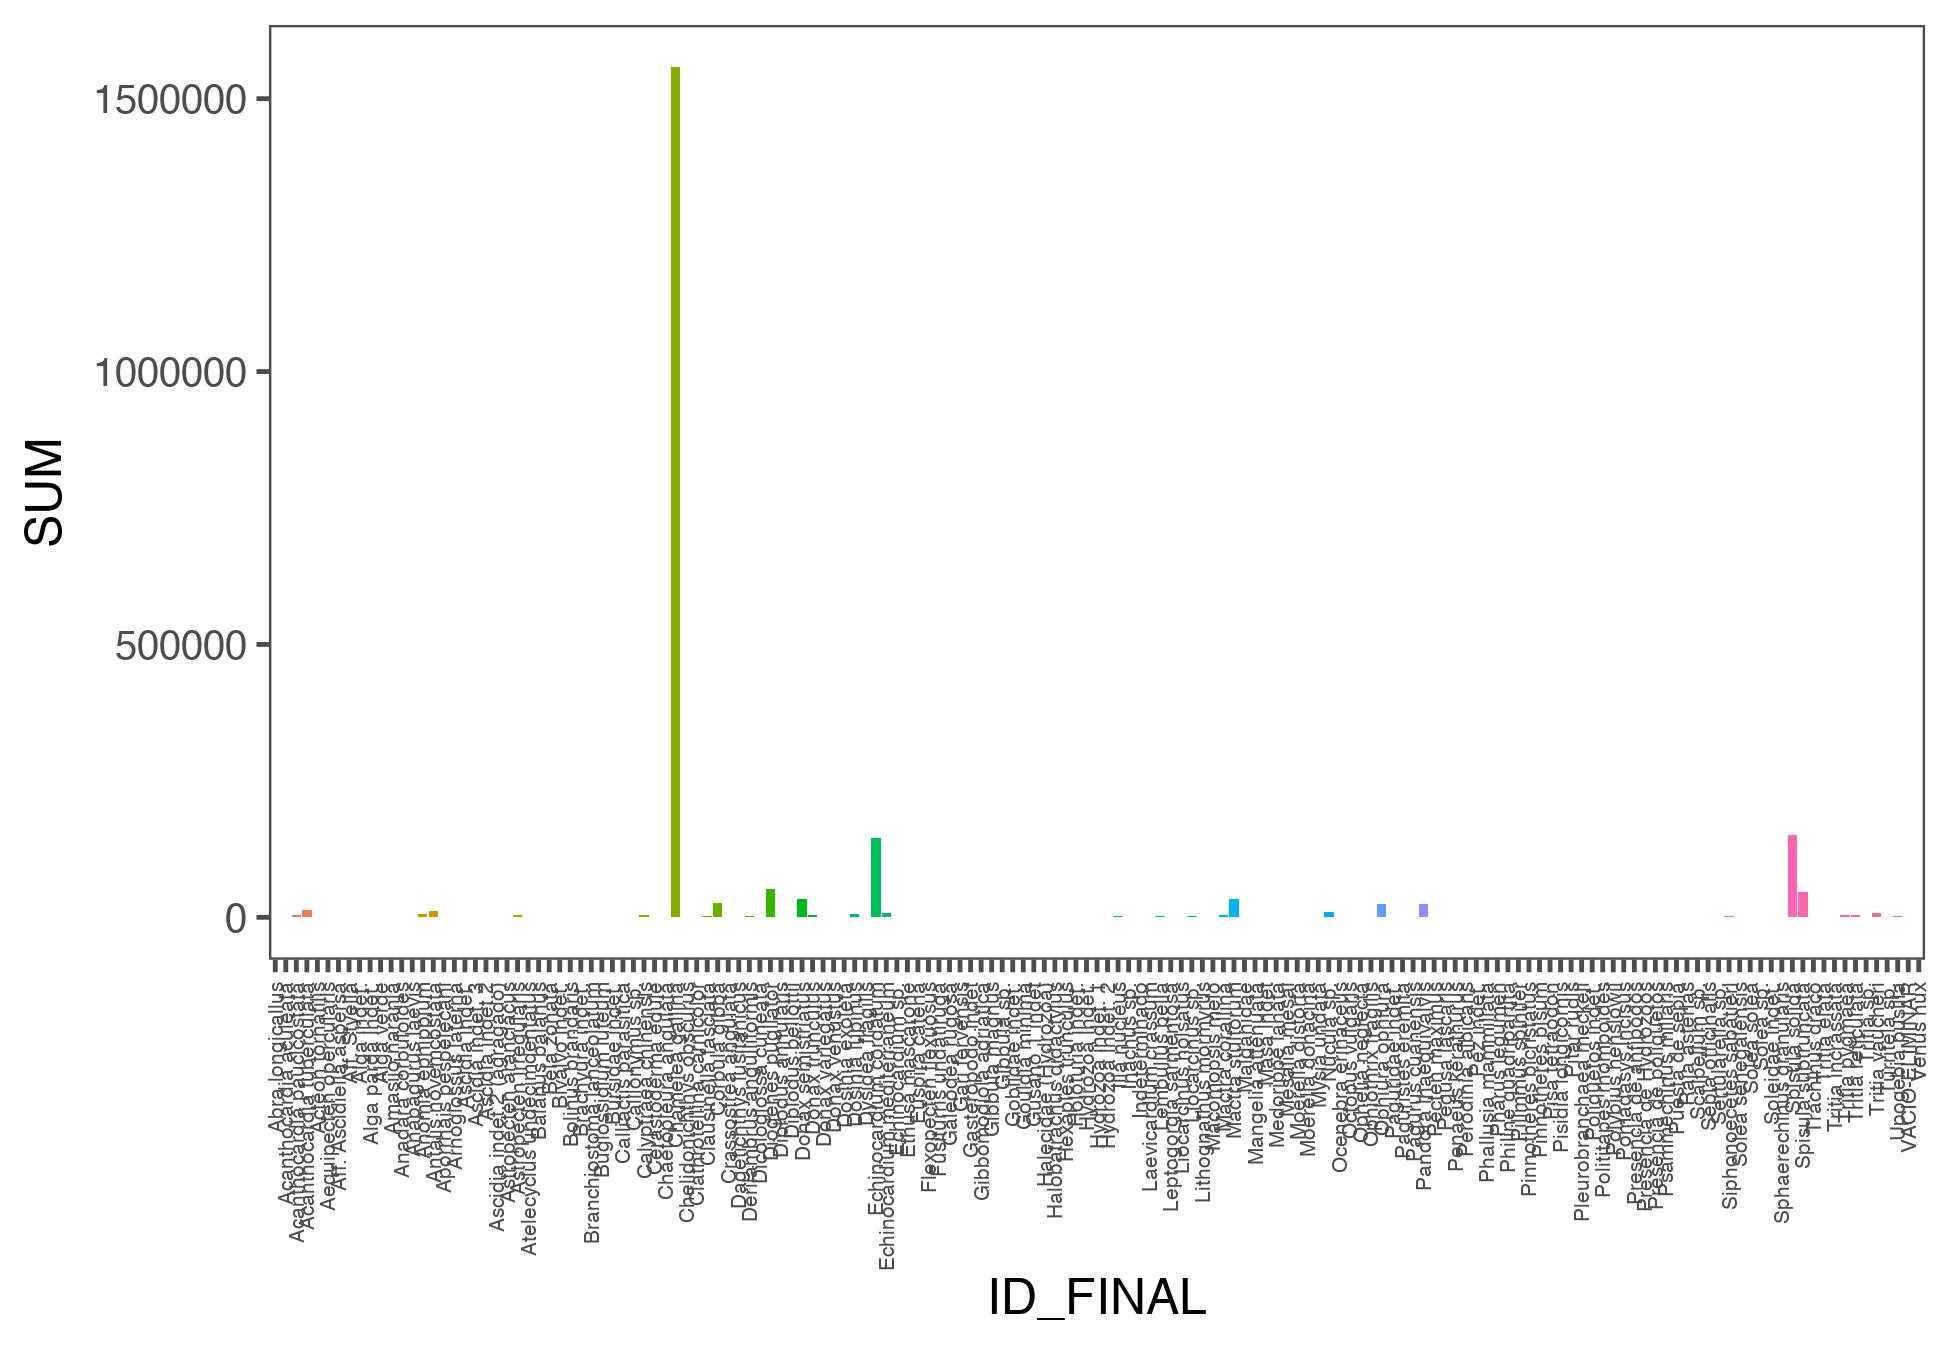
\includegraphics{SAR_Method_files/figure-latex/unnamed-chunk-4-1} \end{center}

\begin{Shaded}
\begin{Highlighting}[]
\NormalTok{pessum}
\end{Highlighting}
\end{Shaded}

\begin{center}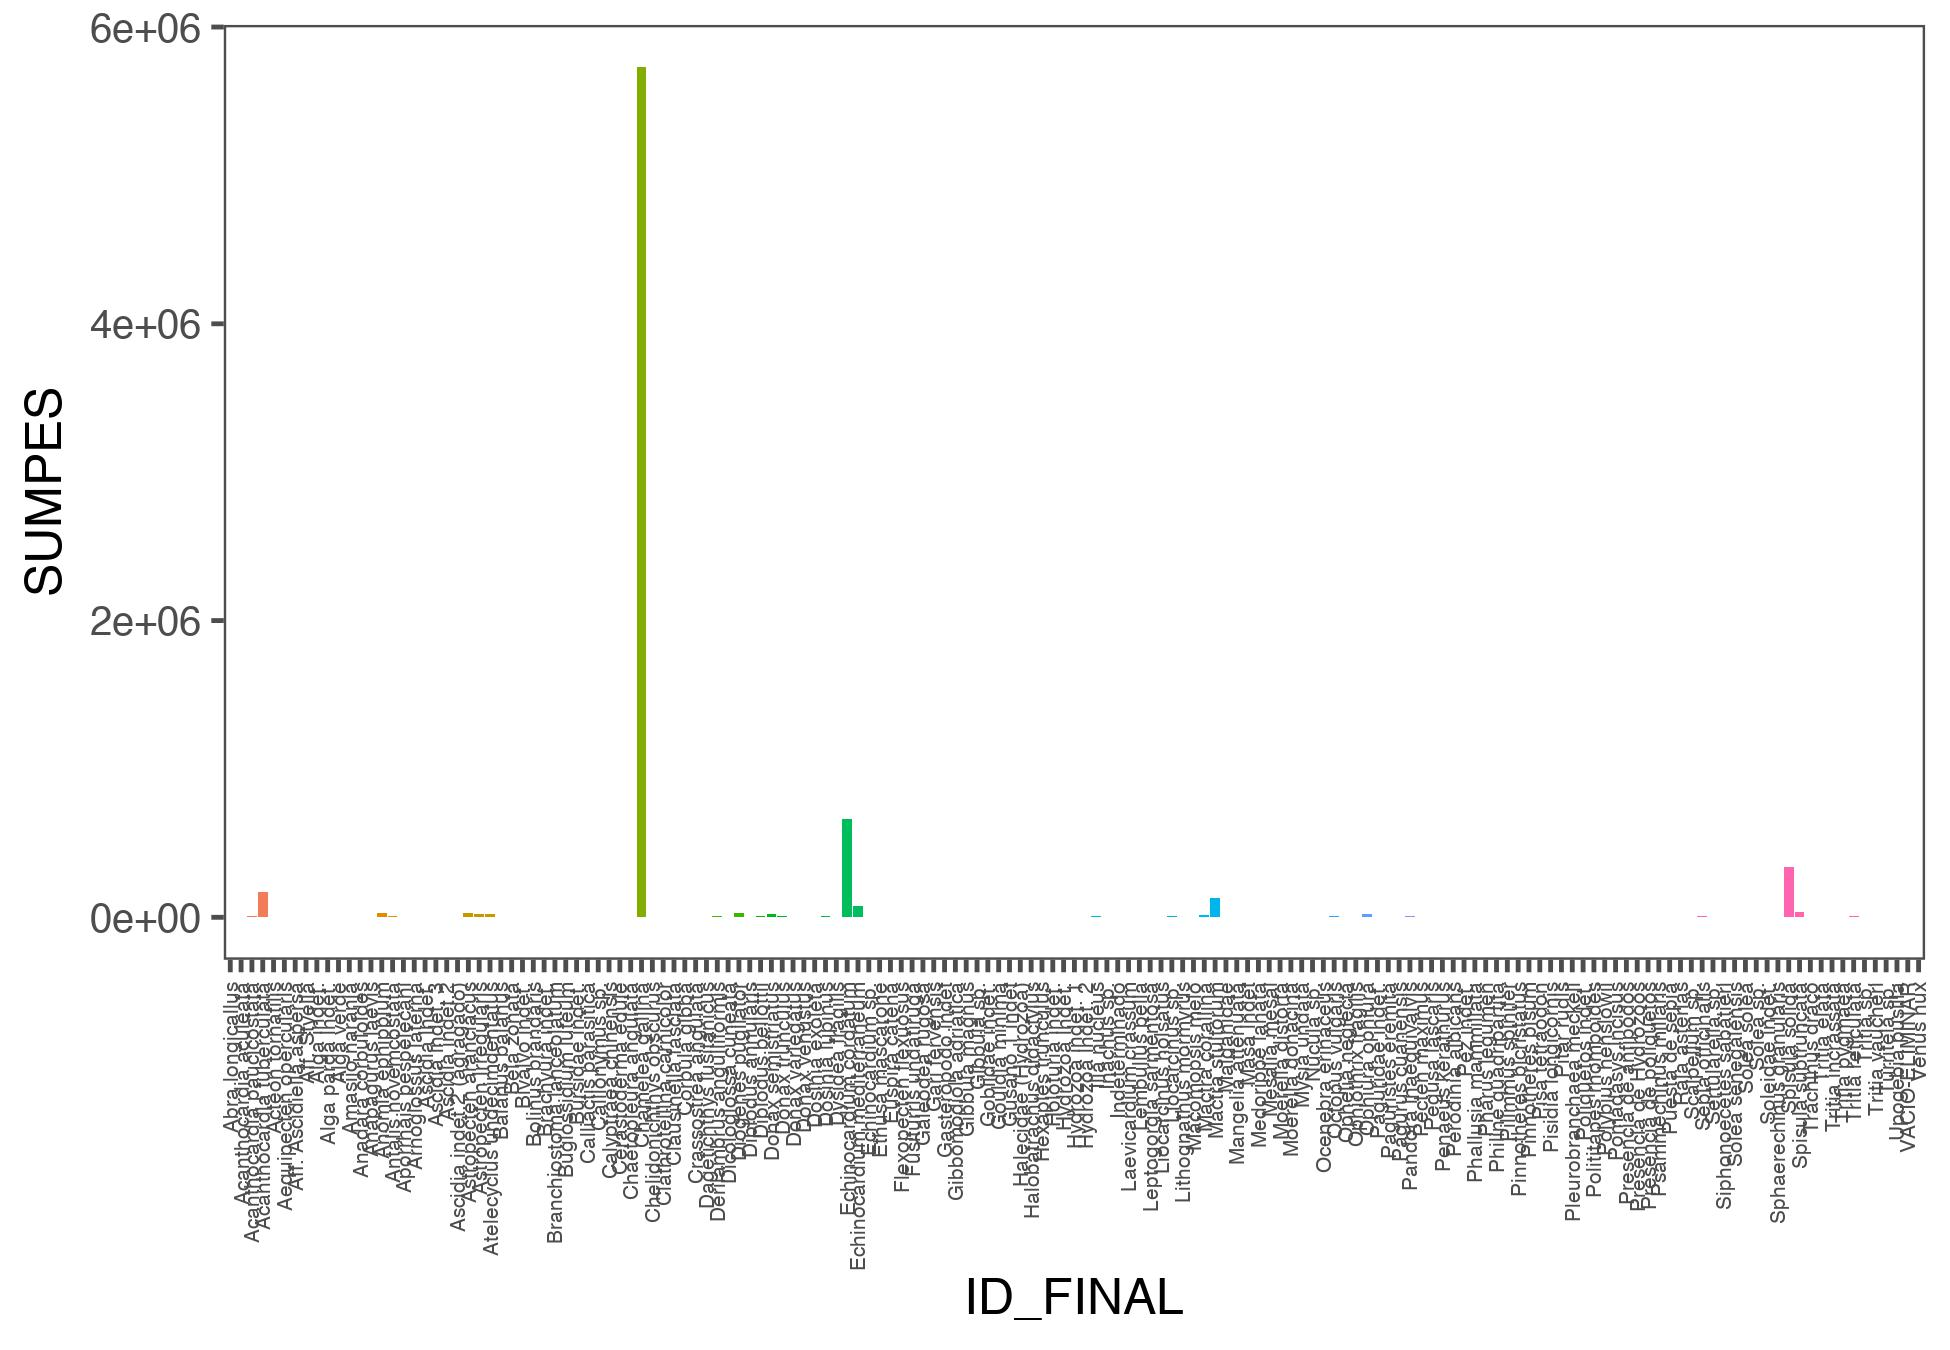
\includegraphics{SAR_Method_files/figure-latex/unnamed-chunk-5-1} \end{center}

\hypertarget{datos-lances}{%
\subsection{Datos Lances}\label{datos-lances}}

\begin{Shaded}
\begin{Highlighting}[]
\NormalTok{setrendi }\OtherTok{\textless{}{-}}\NormalTok{ rendi }\SpecialCharTok{\%\textgreater{}\%} 
  \FunctionTok{group\_by}\NormalTok{()}

\NormalTok{den }\OtherTok{\textless{}{-}} \FunctionTok{ggplot}\NormalTok{(rendi)}\SpecialCharTok{+}
  \FunctionTok{geom\_point}\NormalTok{(}\FunctionTok{aes}\NormalTok{(Estaciones, dens))}\SpecialCharTok{+}
  \FunctionTok{theme\_few}\NormalTok{()}

\NormalTok{bio }\OtherTok{\textless{}{-}} \FunctionTok{ggplot}\NormalTok{(rendi)}\SpecialCharTok{+}
  \FunctionTok{geom\_col}\NormalTok{(}\FunctionTok{aes}\NormalTok{(Estaciones, bio))}\SpecialCharTok{+}
  \FunctionTok{theme\_few}\NormalTok{()}

\NormalTok{ren }\OtherTok{\textless{}{-}} \FunctionTok{ggplot}\NormalTok{(rendi)}\SpecialCharTok{+}
  \FunctionTok{geom\_col}\NormalTok{(}\FunctionTok{aes}\NormalTok{(Estaciones, rend))}\SpecialCharTok{+}
  \FunctionTok{theme\_few}\NormalTok{()}

\NormalTok{area }\OtherTok{\textless{}{-}} \FunctionTok{ggplot}\NormalTok{(rendi)}\SpecialCharTok{+}
  \FunctionTok{geom\_point}\NormalTok{(}\FunctionTok{aes}\NormalTok{(area, rend))}\SpecialCharTok{+}
  \FunctionTok{geom\_smooth}\NormalTok{(}\FunctionTok{aes}\NormalTok{(area, rend))}\SpecialCharTok{+}
  \FunctionTok{theme\_few}\NormalTok{()}

\FunctionTok{ggarrange}\NormalTok{(den, bio , ren, area, }\AttributeTok{ncol=}\DecValTok{2}\NormalTok{)}
\end{Highlighting}
\end{Shaded}

\begin{center}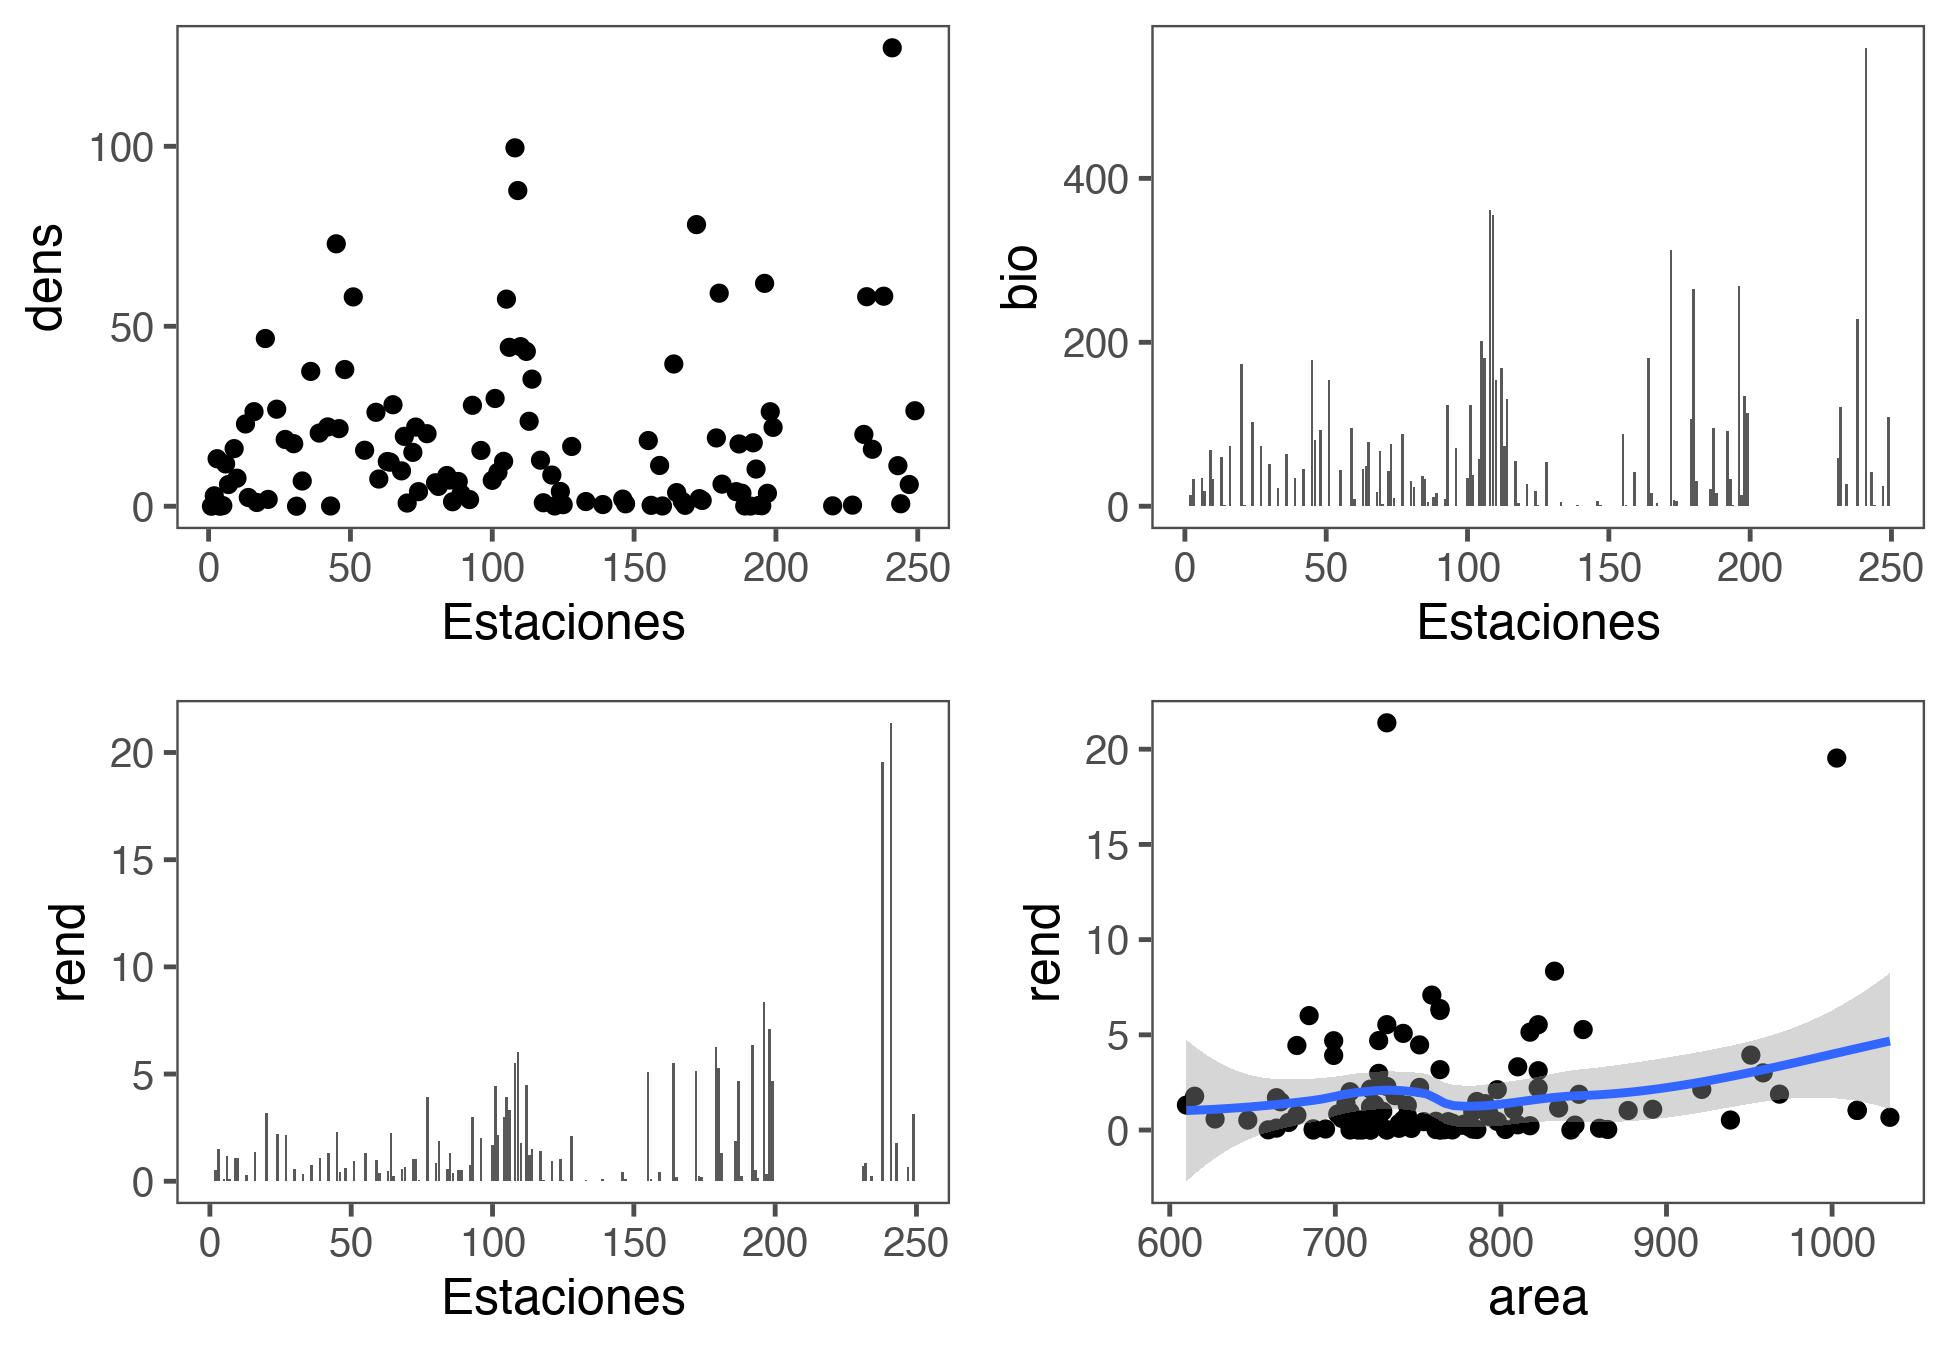
\includegraphics{SAR_Method_files/figure-latex/unnamed-chunk-6-1} \end{center}

Entender las profundidades

\begin{Shaded}
\begin{Highlighting}[]
\NormalTok{f }\OtherTok{\textless{}{-}} \FunctionTok{ggplot}\NormalTok{(rendi)}\SpecialCharTok{+}
  \FunctionTok{geom\_histogram}\NormalTok{(}\FunctionTok{aes}\NormalTok{(depth\_f),}
                 \AttributeTok{binwidth =} \DecValTok{1}\NormalTok{,}
                 \AttributeTok{fill =} \StringTok{"transparent"}\NormalTok{, }\AttributeTok{color =} \StringTok{"red"}\NormalTok{)}\SpecialCharTok{+}
  \FunctionTok{theme\_few}\NormalTok{()}
\NormalTok{i }\OtherTok{\textless{}{-}} \FunctionTok{ggplot}\NormalTok{(rendi)}\SpecialCharTok{+}
  \FunctionTok{geom\_histogram}\NormalTok{(}\FunctionTok{aes}\NormalTok{(depth\_i),}
                 \AttributeTok{binwidth =} \DecValTok{1}\NormalTok{,}
                 \AttributeTok{fill =} \StringTok{"transparent"}\NormalTok{, }\AttributeTok{color =} \StringTok{"blue"}\NormalTok{)}\SpecialCharTok{+}
  \FunctionTok{theme\_few}\NormalTok{()}
\NormalTok{m }\OtherTok{\textless{}{-}} \FunctionTok{ggplot}\NormalTok{(rendi)}\SpecialCharTok{+}
  \FunctionTok{geom\_histogram}\NormalTok{(}\FunctionTok{aes}\NormalTok{(depth\_m),}
                 \AttributeTok{binwidth =} \DecValTok{1}\NormalTok{,}
                 \AttributeTok{fill =} \StringTok{"transparent"}\NormalTok{, }\AttributeTok{color =} \StringTok{"green"}\NormalTok{)}\SpecialCharTok{+}
  \FunctionTok{theme\_few}\NormalTok{()}

\FunctionTok{ggarrange}\NormalTok{(f, i , m , }\AttributeTok{ncol=}\DecValTok{3}\NormalTok{)}
\end{Highlighting}
\end{Shaded}

\begin{center}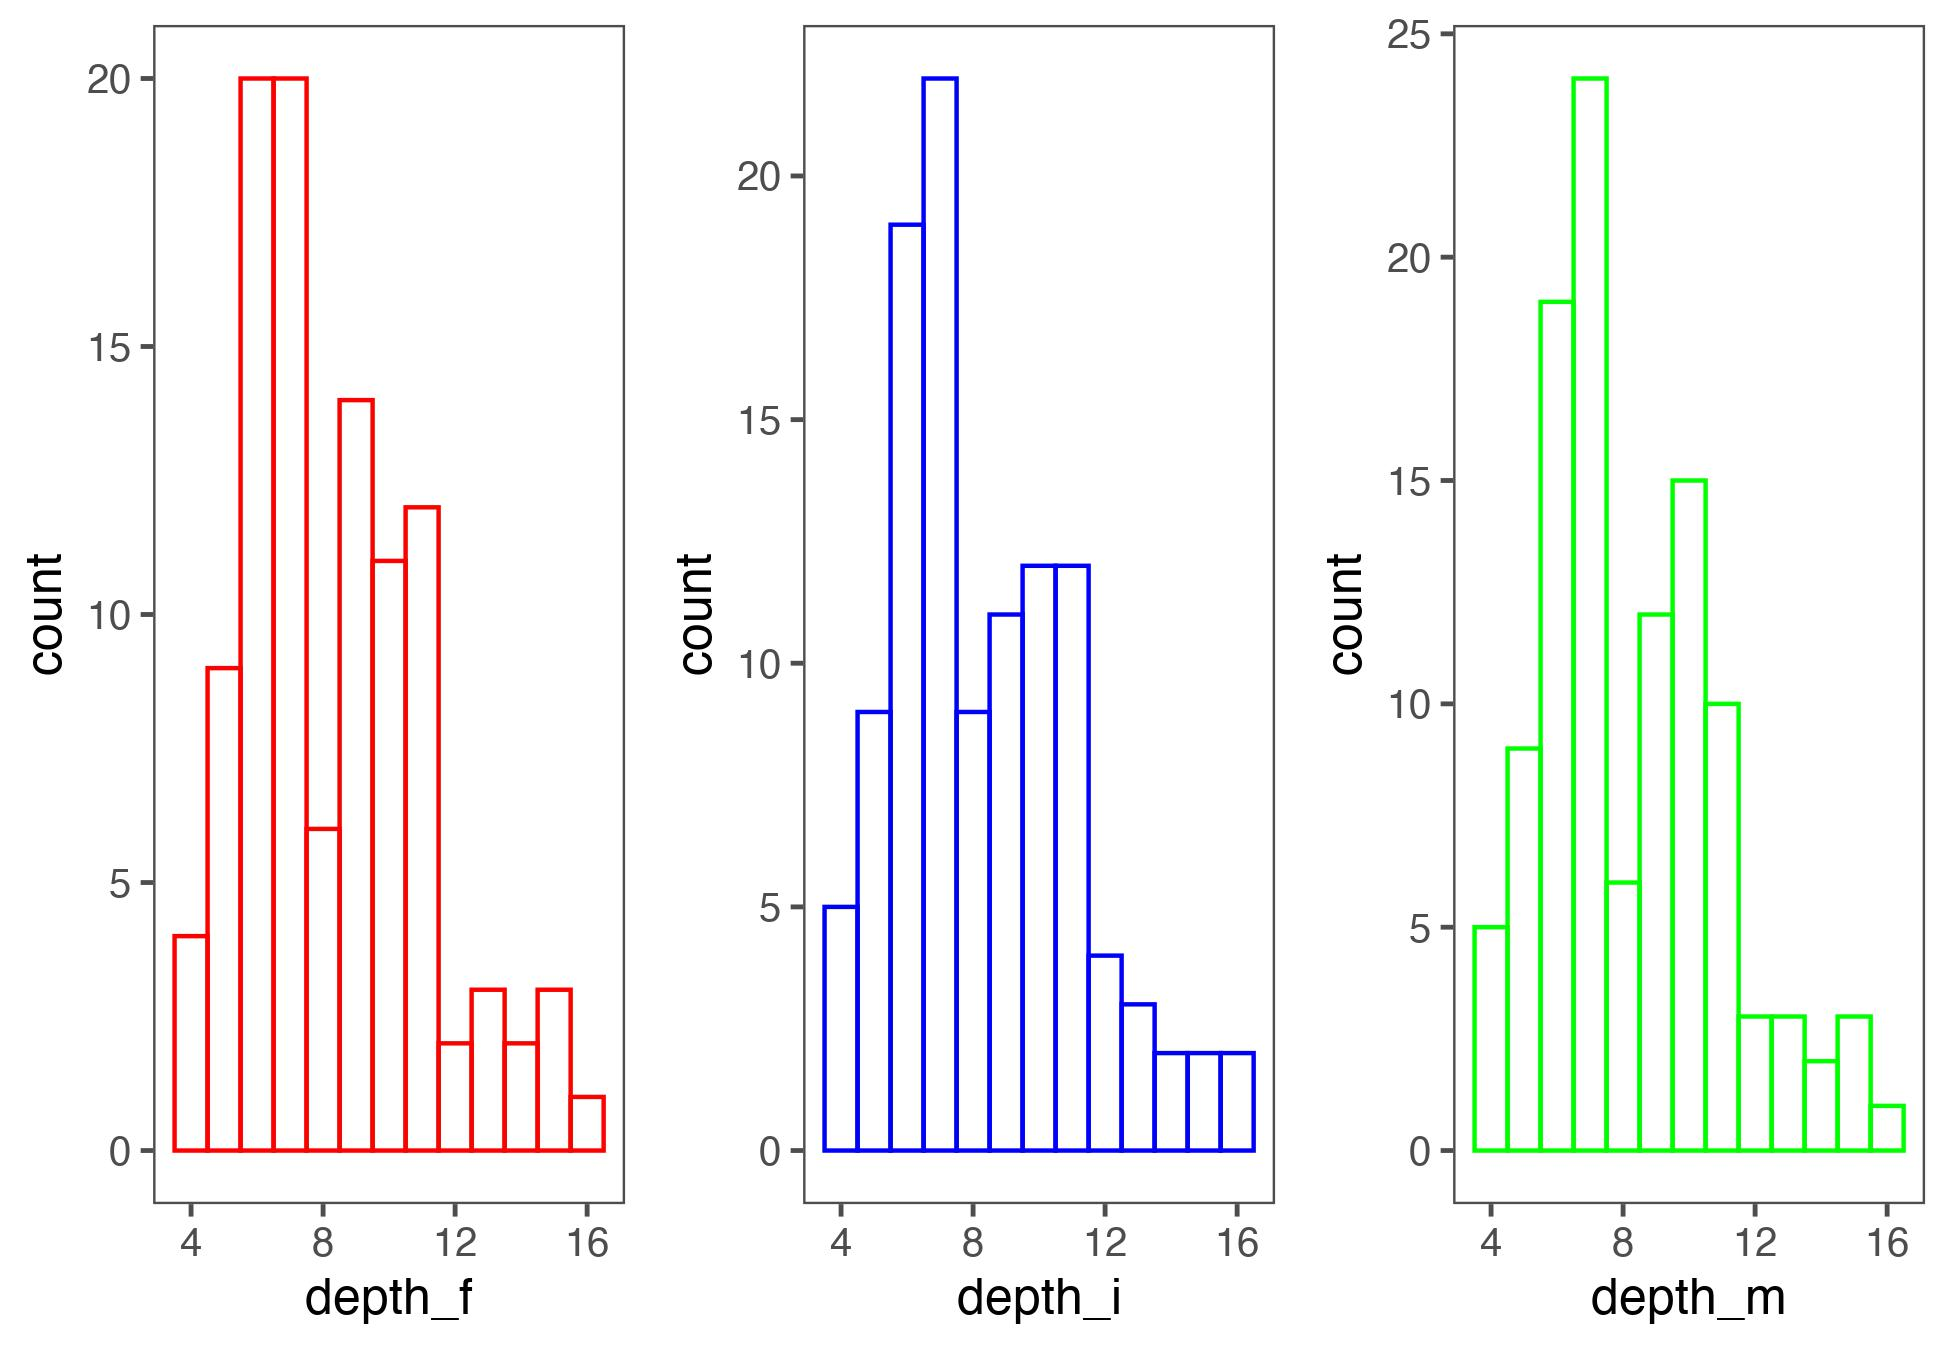
\includegraphics{SAR_Method_files/figure-latex/unnamed-chunk-7-1} \end{center}

\hypertarget{unir-bases}{%
\subsubsection{Unir bases}\label{unir-bases}}

\begin{Shaded}
\begin{Highlighting}[]
\FunctionTok{names}\NormalTok{(fauna)}
\end{Highlighting}
\end{Shaded}

\begin{verbatim}
##  [1] "CAMPAÑA"              "ESTACIÓN"             "CATEGORÍA"           
##  [4] "FECHA"                "PHYLA/Subphylum"      "GRUPO"               
##  [7] "ID_CAMPO"             "ID_FINAL"             "ESTACIÓN + CATEGORÍA"
## [10] "N_ DO...10"           "P_D0...11"            "N_D1...12"           
## [13] "P_D1...13"            "N_D2...14"            "P_D2...15"           
## [16] "N_D3...16"            "P_D3...17"            "Total Indiv...18"    
## [19] "Peso total (g)...19"  "N_ DO...20"           "P_D0...21"           
## [22] "N_D1...22"            "P_D1...23"            "N_D2...24"           
## [25] "P_D2...25"            "N_D3...26"            "P_D3...27"           
## [28] "Total Indiv...28"     "Peso total (g)...29"  "FP"                  
## [31] "N_ DO...31"           "P_D0...32"            "N_D1...33"           
## [34] "P_D1...34"            "N_D2...35"            "P_D2...36"           
## [37] "N_D3...37"            "P_D3...38"            "Total Indiv...39"    
## [40] "Peso total (g)...40"  "N_ DO...41"           "P_D0...42"           
## [43] "N_D1...43"            "P_D1...44"            "N_D2...45"           
## [46] "P_D2...46"            "N_D3...47"            "P_D3...48"           
## [49] "Total Indiv...49"     "Peso total (g)...50"  "%D0"                 
## [52] "%D1"                  "%D2"                  "%D3"                 
## [55] "%DT"
\end{verbatim}

\begin{Shaded}
\begin{Highlighting}[]
\FunctionTok{names}\NormalTok{(station)}
\end{Highlighting}
\end{Shaded}

\begin{verbatim}
## [1] "Estaciones"    "Observaciones" "area"          "station"
\end{verbatim}

\begin{Shaded}
\begin{Highlighting}[]
\FunctionTok{names}\NormalTok{(rendi)}
\end{Highlighting}
\end{Shaded}

\begin{verbatim}
##  [1] "Estaciones"              "Observaciones"          
##  [3] "Date"                    "Track"                  
##  [5] "Track (m)"               "depth_i"                
##  [7] "depth_f"                 "depth_m"                
##  [9] "vel_i"                   "vel_f"                  
## [11] "vel_m"                   "hora_i"                 
## [13] "hora_f"                  "g...14"                 
## [15] "min...15"                "g...16"                 
## [17] "min...17"                "LAT"                    
## [19] "LONG"                    "Nºrejillas"             
## [21] "Vol (l.)...21"           "Vol (l.)...22"          
## [23] "P (total + cascajo) (g)" "SW_tolva"               
## [25] "CSW"                     "CSW_tolva"              
## [27] "N"                       "N_tolva"                
## [29] "area"                    "dens"                   
## [31] "bio"                     "P cascajo (g)"          
## [33] "P cascajo_tolva"         "Tow_time"               
## [35] "PComercial (kg)"         "rend"                   
## [37] "ID"                      "FP"
\end{verbatim}

Cambio el nombre estación en \texttt{fauna}

\begin{Shaded}
\begin{Highlighting}[]
\NormalTok{fauna1 }\OtherTok{\textless{}{-}}\NormalTok{ fauna }\SpecialCharTok{\%\textgreater{}\%} 
  \FunctionTok{rename}\NormalTok{(}\StringTok{"Estaciones"}\OtherTok{=}\StringTok{"ESTACIÓN"}\NormalTok{) }\SpecialCharTok{\%\textgreater{}\%} 
  \FunctionTok{mutate}\NormalTok{(}\AttributeTok{Estaciones =} \FunctionTok{as.double}\NormalTok{(}\FunctionTok{str\_replace}\NormalTok{(Estaciones, }\StringTok{"\^{}E0*"}\NormalTok{, }\StringTok{""}\NormalTok{))) }\SpecialCharTok{\%\textgreater{}\%} 
  \FunctionTok{drop\_na}\NormalTok{(Estaciones)}
\end{Highlighting}
\end{Shaded}

\begin{Shaded}
\begin{Highlighting}[]
\NormalTok{base1  }\OtherTok{\textless{}{-}} \FunctionTok{left\_join}\NormalTok{(rendi, fauna1,}
                   \AttributeTok{by=}\StringTok{"Estaciones"}\NormalTok{)}
\end{Highlighting}
\end{Shaded}

\begin{Shaded}
\begin{Highlighting}[]
\FunctionTok{glimpse}\NormalTok{(base1)}
\end{Highlighting}
\end{Shaded}

\begin{verbatim}
## Rows: 2,119
## Columns: 92
## $ Estaciones                <dbl> 1, 1, 1, 1, 2, 2, 2, 2, 2, 2, 2, 2, 2, 2, 2,~
## $ Observaciones             <chr> NA, NA, NA, NA, NA, NA, NA, NA, NA, NA, NA, ~
## $ Date                      <dttm> 2019-05-06, 2019-05-06, 2019-05-06, 2019-05~
## $ Track                     <chr> ",\"P119-05-06 14:42:4", ",\"P119-05-06 14:4~
## $ `Track (m)`               <dbl> 278, 278, 278, 278, 380, 380, 380, 380, 380,~
## $ depth_i                   <dbl> 4.0, 4.0, 4.0, 4.0, 5.4, 5.4, 5.4, 5.4, 5.4,~
## $ depth_f                   <dbl> 4.0, 4.0, 4.0, 4.0, 3.6, 3.6, 3.6, 3.6, 3.6,~
## $ depth_m                   <dbl> 4.00, 4.00, 4.00, 4.00, 4.50, 4.50, 4.50, 4.~
## $ vel_i                     <dbl> 1.2, 1.2, 1.2, 1.2, 2.0, 2.0, 2.0, 2.0, 2.0,~
## $ vel_f                     <dbl> 1.2, 1.2, 1.2, 1.2, 1.7, 1.7, 1.7, 1.7, 1.7,~
## $ vel_m                     <dbl> 1.20, 1.20, 1.20, 1.20, 1.85, 1.85, 1.85, 1.~
## $ hora_i                    <dttm> 1899-12-31 14:37:17, 1899-12-31 14:37:17, 1~
## $ hora_f                    <dttm> 1899-12-31 14:42:45, 1899-12-31 14:42:45, 1~
## $ g...14                    <dbl> 37, 37, 37, 37, 37, 37, 37, 37, 37, 37, 37, ~
## $ min...15                  <dbl> 9.638, 9.638, 9.638, 9.638, 9.135, 9.135, 9.~
## $ g...16                    <dbl> 7, 7, 7, 7, 7, 7, 7, 7, 7, 7, 7, 7, 7, 7, 7,~
## $ min...17                  <dbl> 23.51, 23.51, 23.51, 23.51, 23.36, 23.36, 23~
## $ LAT                       <dbl> 37.16063, 37.16063, 37.16063, 37.16063, 37.1~
## $ LONG                      <dbl> 7.391833, 7.391833, 7.391833, 7.391833, 7.38~
## $ Nºrejillas                <dbl> 23.0, 23.0, 23.0, 23.0, 6.5, 6.5, 6.5, 6.5, ~
## $ `Vol (l.)...21`           <dbl> 354.19, 354.19, 354.19, 354.19, 97.40, 97.40~
## $ `Vol (l.)...22`           <dbl> 5, 5, 5, 5, 5, 5, 5, 5, 5, 5, 5, 5, 5, 5, 5,~
## $ `P (total + cascajo) (g)` <dbl> 3463.50, 3463.50, 3463.50, 3463.50, 3472.92,~
## $ SW_tolva                  <dbl> 245347.41, 245347.41, 245347.41, 245347.41, ~
## $ CSW                       <dbl> 0.00, 0.00, 0.00, 0.00, 661.76, 661.76, 661.~
## $ CSW_tolva                 <dbl> 0.00, 0.00, 0.00, 0.00, 12891.08, 12891.08, ~
## $ N                         <dbl> 0, 0, 0, 0, 139, 139, 139, 139, 139, 139, 13~
## $ N_tolva                   <dbl> 0.000, 0.000, 0.000, 0.000, 2707.720, 2707.7~
## $ area                      <dbl> 686.66, 686.66, 686.66, 686.66, 938.60, 938.~
## $ dens                      <dbl> 0.00000, 0.00000, 0.00000, 0.00000, 2.88485,~
## $ bio                       <dbl> 0.00000, 0.00000, 0.00000, 0.00000, 13.73438~
## $ `P cascajo (g)`           <lgl> NA, NA, NA, NA, NA, NA, NA, NA, NA, NA, NA, ~
## $ `P cascajo_tolva`         <lgl> NA, NA, NA, NA, NA, NA, NA, NA, NA, NA, NA, ~
## $ Tow_time                  <dttm> 1899-12-31 00:05:28, 1899-12-31 00:05:28, 1~
## $ `PComercial (kg)`         <dbl> 0.00000, 0.00000, 0.00000, 0.00000, 2.62219,~
## $ rend                      <dbl> 0.000000, 0.000000, 0.000000, 0.000000, 0.52~
## $ ID                        <dbl> 1, 1, 1, 1, 2, 2, 2, 2, 2, 2, 2, 2, 2, 2, 2,~
## $ FP.x                      <dbl> 70.838, 70.838, 70.838, 70.838, 19.480, 19.4~
## $ CAMPAÑA                   <chr> "ACUVEN-3D", "ACUVEN-3D", "ACUVEN-3D", "ACUV~
## $ CATEGORÍA                 <chr> "POBLACIONAL", "POBLACIONAL", "POBLACIONAL",~
## $ FECHA                     <dttm> 2019-05-06, 2019-05-06, 2019-05-06, 2019-05~
## $ `PHYLA/Subphylum`         <chr> "ANNELIDA", "ECHINODERMATA", "MOLLUSCA", "MO~
## $ GRUPO                     <chr> "POLYCHAETA", "ECHINOIDEA", "BIVALVIA", "BIV~
## $ ID_CAMPO                  <chr> "Poliquetos indet.", "Echinocardium mediterr~
## $ ID_FINAL                  <chr> "Ophelia neglecta", "Echinocardium mediterra~
## $ `ESTACIÓN + CATEGORÍA`    <chr> "E1", "E1", "E1", "E1", "E2", "E2-CAPTURA TO~
## $ `N_ DO...10`              <dbl> 1, 6, 14, 3, NA, NA, 2, 19, NA, 1, 73, NA, 2~
## $ P_D0...11                 <dbl> 0.290, 83.040, 38.540, 5.580, 9.190, NA, 2.7~
## $ N_D1...12                 <dbl> NA, NA, NA, NA, NA, NA, NA, NA, 2, NA, NA, N~
## $ P_D1...13                 <dbl> NA, NA, NA, NA, NA, NA, NA, NA, 9.24, NA, NA~
## $ N_D2...14                 <dbl> NA, NA, NA, NA, NA, NA, NA, NA, NA, NA, NA, ~
## $ P_D2...15                 <dbl> NA, NA, NA, NA, NA, NA, NA, NA, NA, NA, NA, ~
## $ N_D3...16                 <dbl> NA, 3, NA, NA, NA, NA, NA, NA, NA, NA, 107, ~
## $ P_D3...17                 <dbl> NA, 47.88, NA, NA, NA, NA, NA, NA, NA, NA, 9~
## $ `Total Indiv...18`        <dbl> 1, 9, 14, 3, 0, NA, 2, 19, 2, 1, 180, NA, 3,~
## $ `Peso total (g)...19`     <dbl> 0.290, 130.920, 38.540, 5.580, 9.190, NA, 2.~
## $ `N_ DO...20`              <dbl> NA, NA, NA, NA, NA, 1, NA, NA, NA, NA, NA, 1~
## $ P_D0...21                 <chr> NA, NA, NA, NA, NA, "249.34", NA, NA, NA, NA~
## $ N_D1...22                 <dbl> NA, NA, NA, NA, NA, NA, NA, NA, 1, NA, NA, N~
## $ P_D1...23                 <dbl> NA, NA, NA, NA, NA, NA, NA, NA, 4.34, NA, NA~
## $ N_D2...24                 <dbl> NA, NA, NA, NA, NA, NA, NA, NA, NA, NA, NA, ~
## $ P_D2...25                 <dbl> NA, NA, NA, NA, NA, NA, NA, NA, NA, NA, NA, ~
## $ N_D3...26                 <dbl> NA, NA, NA, NA, NA, NA, NA, NA, 1, NA, NA, N~
## $ P_D3...27                 <dbl> NA, NA, NA, NA, NA, NA, NA, NA, 6.35, NA, NA~
## $ `Total Indiv...28`        <dbl> NA, NA, NA, NA, NA, 1, NA, NA, 2, NA, NA, 1,~
## $ `Peso total (g)...29`     <dbl> NA, NA, NA, NA, NA, 249.34, NA, NA, 10.69, N~
## $ FP.y                      <dbl> 70.84, 70.84, 70.84, 70.84, 19.48, 19.48, 19~
## $ `N_ DO...31`              <dbl> 70.84, 425.04, 991.76, 212.52, 0.00, 0.00, 3~
## $ P_D0...32                 <dbl> 20.54360, 5882.55360, 2730.17360, 395.28720,~
## $ N_D1...33                 <dbl> 0.00, 0.00, 0.00, 0.00, 0.00, 0.00, 0.00, 0.~
## $ P_D1...34                 <dbl> 0.0000, 0.0000, 0.0000, 0.0000, 0.0000, 0.00~
## $ N_D2...35                 <dbl> 0, 0, 0, 0, 0, 0, 0, 0, 0, 0, 0, 0, 0, 0, 0,~
## $ P_D2...36                 <dbl> 0, 0, 0, 0, 0, 0, 0, 0, 0, 0, 0, 0, 0, 0, 0,~
## $ N_D3...37                 <dbl> 0.00, 212.52, 0.00, 0.00, 0.00, 0.00, 0.00, ~
## $ P_D3...38                 <dbl> 0.0000, 3391.8192, 0.0000, 0.0000, 0.0000, 0~
## $ `Total Indiv...39`        <dbl> 70.84, 637.56, 991.76, 212.52, 0.00, 0.00, 3~
## $ `Peso total (g)...40`     <dbl> 20.54360, 9274.37280, 2730.17360, 395.28720,~
## $ `N_ DO...41`              <dbl> 70.84, 425.04, 991.76, 212.52, 0.00, 1.00, 3~
## $ P_D0...42                 <dbl> 20.54360, 5882.55360, 2730.17360, 395.28720,~
## $ N_D1...43                 <dbl> 0.00, 0.00, 0.00, 0.00, 0.00, 0.00, 0.00, 0.~
## $ P_D1...44                 <dbl> 0.0000, 0.0000, 0.0000, 0.0000, 0.0000, 0.00~
## $ N_D2...45                 <dbl> 0, 0, 0, 0, 0, 0, 0, 0, 0, 0, 0, 0, 0, 0, 0,~
## $ P_D2...46                 <dbl> 0, 0, 0, 0, 0, 0, 0, 0, 0, 0, 0, 0, 0, 0, 0,~
## $ N_D3...47                 <dbl> 0.00, 212.52, 0.00, 0.00, 0.00, 0.00, 0.00, ~
## $ P_D3...48                 <dbl> 0.0000, 3391.8192, 0.0000, 0.0000, 0.0000, 0~
## $ `Total Indiv...49`        <dbl> 70.84, 637.56, 991.76, 212.52, 0.00, 1.00, 3~
## $ `Peso total (g)...50`     <dbl> 20.54360, 9274.37280, 2730.17360, 395.28720,~
## $ `%D0`                     <dbl> 100.00000, 66.66667, 100.00000, 100.00000, N~
## $ `%D1`                     <dbl> 0.00000, 0.00000, 0.00000, 0.00000, NA, 0.00~
## $ `%D2`                     <dbl> 0, 0, 0, 0, NA, 0, 0, 0, 0, 0, 0, 0, 0, 0, 0~
## $ `%D3`                     <dbl> 0.000000, 33.333333, 0.000000, 0.000000, NA,~
## $ `%DT`                     <dbl> 0.000000, 33.333333, 0.000000, 0.000000, NA,~
\end{verbatim}

\hypertarget{data-caja-verdes}{%
\subsection{Data Caja Verdes}\label{data-caja-verdes}}

Por ahora solo trabajaremos con la data entregada por Candelaria Burgos para Chirla, que son los datos del año 2008 y 2009.

\begin{Shaded}
\begin{Highlighting}[]
\NormalTok{cajas2009 }\OtherTok{\textless{}{-}} \FunctionTok{c}\NormalTok{(}\StringTok{"Draga\_01\_2009.txt"}\NormalTok{,}
           \StringTok{"Draga\_02\_2009.txt"}\NormalTok{,}
           \StringTok{"Draga\_03\_2009.txt"}\NormalTok{, }
           \StringTok{"Draga\_04\_2009.txt"}\NormalTok{ ,}
           \StringTok{"Draga\_05\_2008.txt"}\NormalTok{ ,}
           \StringTok{"Draga\_06\_2008.txt"}\NormalTok{,}
           \StringTok{"Draga\_07\_2008.txt"}\NormalTok{ ,}
           \StringTok{"Draga\_08\_2008.txt"}\NormalTok{,}
           \StringTok{"Draga\_09\_2008.txt"}\NormalTok{ ,}
           \StringTok{"Draga\_10\_2008.txt"}\NormalTok{,}
           \StringTok{"Draga\_11\_2008.txt"}\NormalTok{ ,}
           \StringTok{"Draga\_12\_2008.txt"}\NormalTok{)}
\NormalTok{caja1 }\OtherTok{\textless{}{-}} \FunctionTok{read.table}\NormalTok{(}\FunctionTok{here}\NormalTok{(}\StringTok{"DATOS"}\NormalTok{,}
                         \StringTok{"Cajas verdes chirla"}\NormalTok{,}
                         \StringTok{"Draga\_2008\_2009"}\NormalTok{,}
                         \StringTok{"Draga\_01\_2009.txt"}\NormalTok{), }
                     \AttributeTok{sep =} \StringTok{";"}\NormalTok{,}
                    \AttributeTok{header =} \ConstantTok{TRUE}\NormalTok{)}

\CommentTok{\# Lista para almacenar los datos}
\NormalTok{lista\_datos }\OtherTok{\textless{}{-}} \FunctionTok{list}\NormalTok{()}
\CommentTok{\# Ciclo for para leer cada archivo}
\ControlFlowTok{for}\NormalTok{ (archivo }\ControlFlowTok{in}\NormalTok{ cajas2009) \{}
  \CommentTok{\# Ruta completa del archivo}
\NormalTok{  ruta }\OtherTok{\textless{}{-}} \FunctionTok{here}\NormalTok{(}\StringTok{"DATOS"}\NormalTok{, }
               \StringTok{"Cajas verdes chirla"}\NormalTok{,}
               \StringTok{"Draga\_2008\_2009"}\NormalTok{, archivo)}
  \CommentTok{\# Leer el archivo y agregarlo a la lista}
\NormalTok{  datos }\OtherTok{\textless{}{-}} \FunctionTok{read.table}\NormalTok{(ruta, }\AttributeTok{sep =} \StringTok{";"}\NormalTok{, }\AttributeTok{header =} \ConstantTok{TRUE}\NormalTok{)}
\NormalTok{  lista\_datos[[archivo]] }\OtherTok{\textless{}{-}}\NormalTok{ datos}
\NormalTok{\}}
\end{Highlighting}
\end{Shaded}

\begin{Shaded}
\begin{Highlighting}[]
\NormalTok{cajas2009uni }\OtherTok{\textless{}{-}} \FunctionTok{do.call}\NormalTok{(rbind, }
\NormalTok{                        lista\_datos)}
\end{Highlighting}
\end{Shaded}

Verifico la dimension de la base

\begin{Shaded}
\begin{Highlighting}[]
\FunctionTok{dim}\NormalTok{(cajas2009uni)}
\end{Highlighting}
\end{Shaded}

\begin{verbatim}
## [1] 1554983      21
\end{verbatim}

calculo la cantidad de embarcaciones presentes en la BD

\begin{Shaded}
\begin{Highlighting}[]
\FunctionTok{unique}\NormalTok{(cajas2009uni}\SpecialCharTok{$}\NormalTok{MATRICULA)}
\end{Highlighting}
\end{Shaded}

\begin{verbatim}
##  [1] "SE-1-768"   "HU-2-2158"  "HU-2-1931"  "SE-1-792"   "HU-3-1512" 
##  [6] "HU-2-2207"  "HU-3-5-91"  "AL-2-1833"  "HU-2-1-95"  "SE-1-1-95" 
## [11] "HU-2-3-95"  "HU-2-2-95"  "HU-1-5-96"  "HU-2-7-97"  "HU-2-1-97" 
## [16] "HU-2-5-96"  "HU-2-3-96"  "HU-2-3-98"  "HU-3-11-98" "HU-2-4-98" 
## [21] "HU-2-3-97"  "SE-1-4-98"  "HU-3-3-99"  "HU-2-8-98"  "HU-3-2-99" 
## [26] "HU-2-3-99"  "HU-2-8-99"  "HU-2-9-99"  "HU-2-13-99" "HU-2-14-99"
## [31] "HU-2-8-00"  "HU-3-8-00"  "HU-3-10-00" "HU-3-1-01"  "HU-2-5-01" 
## [36] "HU-2-9-01"  "HU-3-4-01"  "HU-3-13-00" "HU-2-17-01" "SE-1-8-01" 
## [41] "HU-2-7-01"  "HU-3-1-02"  "HU-2-28-01" "HU-2-7-02"  "HU-2-8-02" 
## [46] "HU-2-16-02" "HU-2-17-02" "HU-3-9-02"  "HU-3-14-02" "HU-3-6-02" 
## [51] "HU-3-4-02"  "SE-1-10-03" "HU-3-12-02" "HU-2-14-03" "HU-3-11-02"
## [56] "HU-2-27-03" "HU-2-29-03" "HU-2-5-04"  "HU-3-1-04"  "HU-2-9-04" 
## [61] "HU-1-3-04"  "HU-3-8-04"  "HU-1-4-05"  "HU-2-13-05" "HU-3-2-04" 
## [66] "HU-3-7-05"  "HU-3-2-05"  "HU-3-4-05"  "HU-3-9-05"  "HU-3-8-05" 
## [71] "HU-3-6-04"  "HU-3-1-06"  "HU-2-4-06"  "HU-3-5-05"  "HU-3-5-06" 
## [76] "HU-2-2-07"  "HU-3-1164"  "HU-2-8-97"  "HU-2-11-99" "HU-2-19-01"
## [81] "SE-1-14-04" "HU-2-1-06"  "HU-2-2-06"  "SE-1-15-03" "HU-3-5-02" 
## [86] "HU-2-15-01" "HU-2-13-02" "HU-3-16-02" "HU-2-1218"  "HU-2-12-02"
## [91] "SE-1-14-03" "HU-3-10-04" "HU-2-8-01"
\end{verbatim}

cambio el formato de fechas:

\begin{Shaded}
\begin{Highlighting}[]
\NormalTok{cajas2009uni}\SpecialCharTok{$}\NormalTok{FECHA }\OtherTok{\textless{}{-}} \FunctionTok{ymd}\NormalTok{(cajas2009uni}\SpecialCharTok{$}\NormalTok{FECHA) }


\NormalTok{cajassep }\OtherTok{\textless{}{-}}\NormalTok{ cajas2009uni }\SpecialCharTok{\%\textgreater{}\%}
  \FunctionTok{mutate}\NormalTok{(}\AttributeTok{ANO =} \FunctionTok{year}\NormalTok{(FECHA),}
         \AttributeTok{MES =} \FunctionTok{month}\NormalTok{(FECHA),}
         \AttributeTok{DIA =} \FunctionTok{day}\NormalTok{(FECHA))}
\end{Highlighting}
\end{Shaded}

De forma simple compruenbo los meses y dias con actividad de los datos sin filtrar;

\begin{Shaded}
\begin{Highlighting}[]
\NormalTok{diahis }\OtherTok{\textless{}{-}} \FunctionTok{ggplot}\NormalTok{()}\SpecialCharTok{+}
  \FunctionTok{geom\_histogram}\NormalTok{(}\FunctionTok{aes}\NormalTok{(cajassep}\SpecialCharTok{$}\NormalTok{DIA), }
                     \AttributeTok{col=}\DecValTok{2}\NormalTok{,}
                     \AttributeTok{fill=}\StringTok{"white"}\NormalTok{,}
                 \AttributeTok{binwidth =} \DecValTok{1}\NormalTok{)}\SpecialCharTok{+}
  \FunctionTok{theme\_few}\NormalTok{()}
\NormalTok{meshis }\OtherTok{\textless{}{-}} \FunctionTok{ggplot}\NormalTok{()}\SpecialCharTok{+}
  \FunctionTok{geom\_histogram}\NormalTok{(}\FunctionTok{aes}\NormalTok{(cajassep}\SpecialCharTok{$}\NormalTok{MES), }
                     \AttributeTok{col=}\DecValTok{3}\NormalTok{,}
                     \AttributeTok{fill=}\StringTok{"white"}\NormalTok{,}
                 \AttributeTok{binwidth =} \DecValTok{1}\NormalTok{)}\SpecialCharTok{+}
  \FunctionTok{theme\_few}\NormalTok{()}
\NormalTok{velhis }\OtherTok{\textless{}{-}} \FunctionTok{ggplot}\NormalTok{()}\SpecialCharTok{+}
  \FunctionTok{geom\_histogram}\NormalTok{(}\FunctionTok{aes}\NormalTok{(cajassep}\SpecialCharTok{$}\NormalTok{N\_VELOCIDAD), }
                     \AttributeTok{col=}\DecValTok{4}\NormalTok{,}
                     \AttributeTok{fill=}\StringTok{"white"}\NormalTok{,}
                 \AttributeTok{binwidth =} \FloatTok{0.1}\NormalTok{)}\SpecialCharTok{+}
  \FunctionTok{theme\_few}\NormalTok{()}
\FunctionTok{ggarrange}\NormalTok{(diahis, meshis, velhis, }\AttributeTok{ncol=}\DecValTok{3}\NormalTok{)}
\end{Highlighting}
\end{Shaded}

Los métodos para la estimación y cartografiado del esfuerzo pesquero a partir de los datos de los VMS ya se han estudiado en varias pesquerías anteriormente. Estos estudios recomiendan un proceso en varios pasos según (\protect\hyperlink{ref-Cojan2012}{\textbf{Cojan2012?}}):

1- Borrar los registros duplicados,

\begin{Shaded}
\begin{Highlighting}[]
\CommentTok{\# Encontrar filas duplicadas}
\NormalTok{filas\_duplicadas }\OtherTok{\textless{}{-}} \FunctionTok{duplicated}\NormalTok{(cajassep)}
\CommentTok{\# Mostrar las filas duplicadas}
\NormalTok{datos\_duplicados }\OtherTok{\textless{}{-}}\NormalTok{ cajassep[filas\_duplicadas, ]}

\CommentTok{\# Opcionalmente, para eliminar filas duplicadas manteniendo solo la última ocurrencia de cada fila duplicada:}
\NormalTok{cajasfil }\OtherTok{\textless{}{-}}\NormalTok{ cajassep[}\SpecialCharTok{!}\FunctionTok{duplicated}\NormalTok{(cajassep, }
                                 \AttributeTok{fromLast =} \ConstantTok{TRUE}\NormalTok{), ]}
\end{Highlighting}
\end{Shaded}

2- Borrar los registros en puertos.

\begin{Shaded}
\begin{Highlighting}[]
\NormalTok{cajasfilp }\OtherTok{\textless{}{-}}\NormalTok{ cajasfil }\SpecialCharTok{\%\textgreater{}\%} 
  \FunctionTok{filter}\NormalTok{(N\_EN\_PUERTO }\SpecialCharTok{==} \DecValTok{0}\NormalTok{)}
\end{Highlighting}
\end{Shaded}

\begin{Shaded}
\begin{Highlighting}[]
\NormalTok{velhis }\OtherTok{\textless{}{-}} \FunctionTok{ggplot}\NormalTok{()}\SpecialCharTok{+}
  \FunctionTok{geom\_histogram}\NormalTok{(}\FunctionTok{aes}\NormalTok{(cajasfilp}\SpecialCharTok{$}\NormalTok{N\_VELOCIDAD,}
                     \AttributeTok{fill=}\NormalTok{cajasfilp}\SpecialCharTok{$}\NormalTok{N\_VELOCIDAD }\SpecialCharTok{\textless{}} \FloatTok{1.5}\NormalTok{),}
                 \AttributeTok{binwidth =} \FloatTok{0.02}\NormalTok{)}\SpecialCharTok{+}
  \FunctionTok{scale\_fill\_viridis\_d}\NormalTok{()}\SpecialCharTok{+}
  \FunctionTok{theme}\NormalTok{(}\AttributeTok{legend.position =} \StringTok{"none"}\NormalTok{)}
\NormalTok{velhis}
\end{Highlighting}
\end{Shaded}

\begin{center}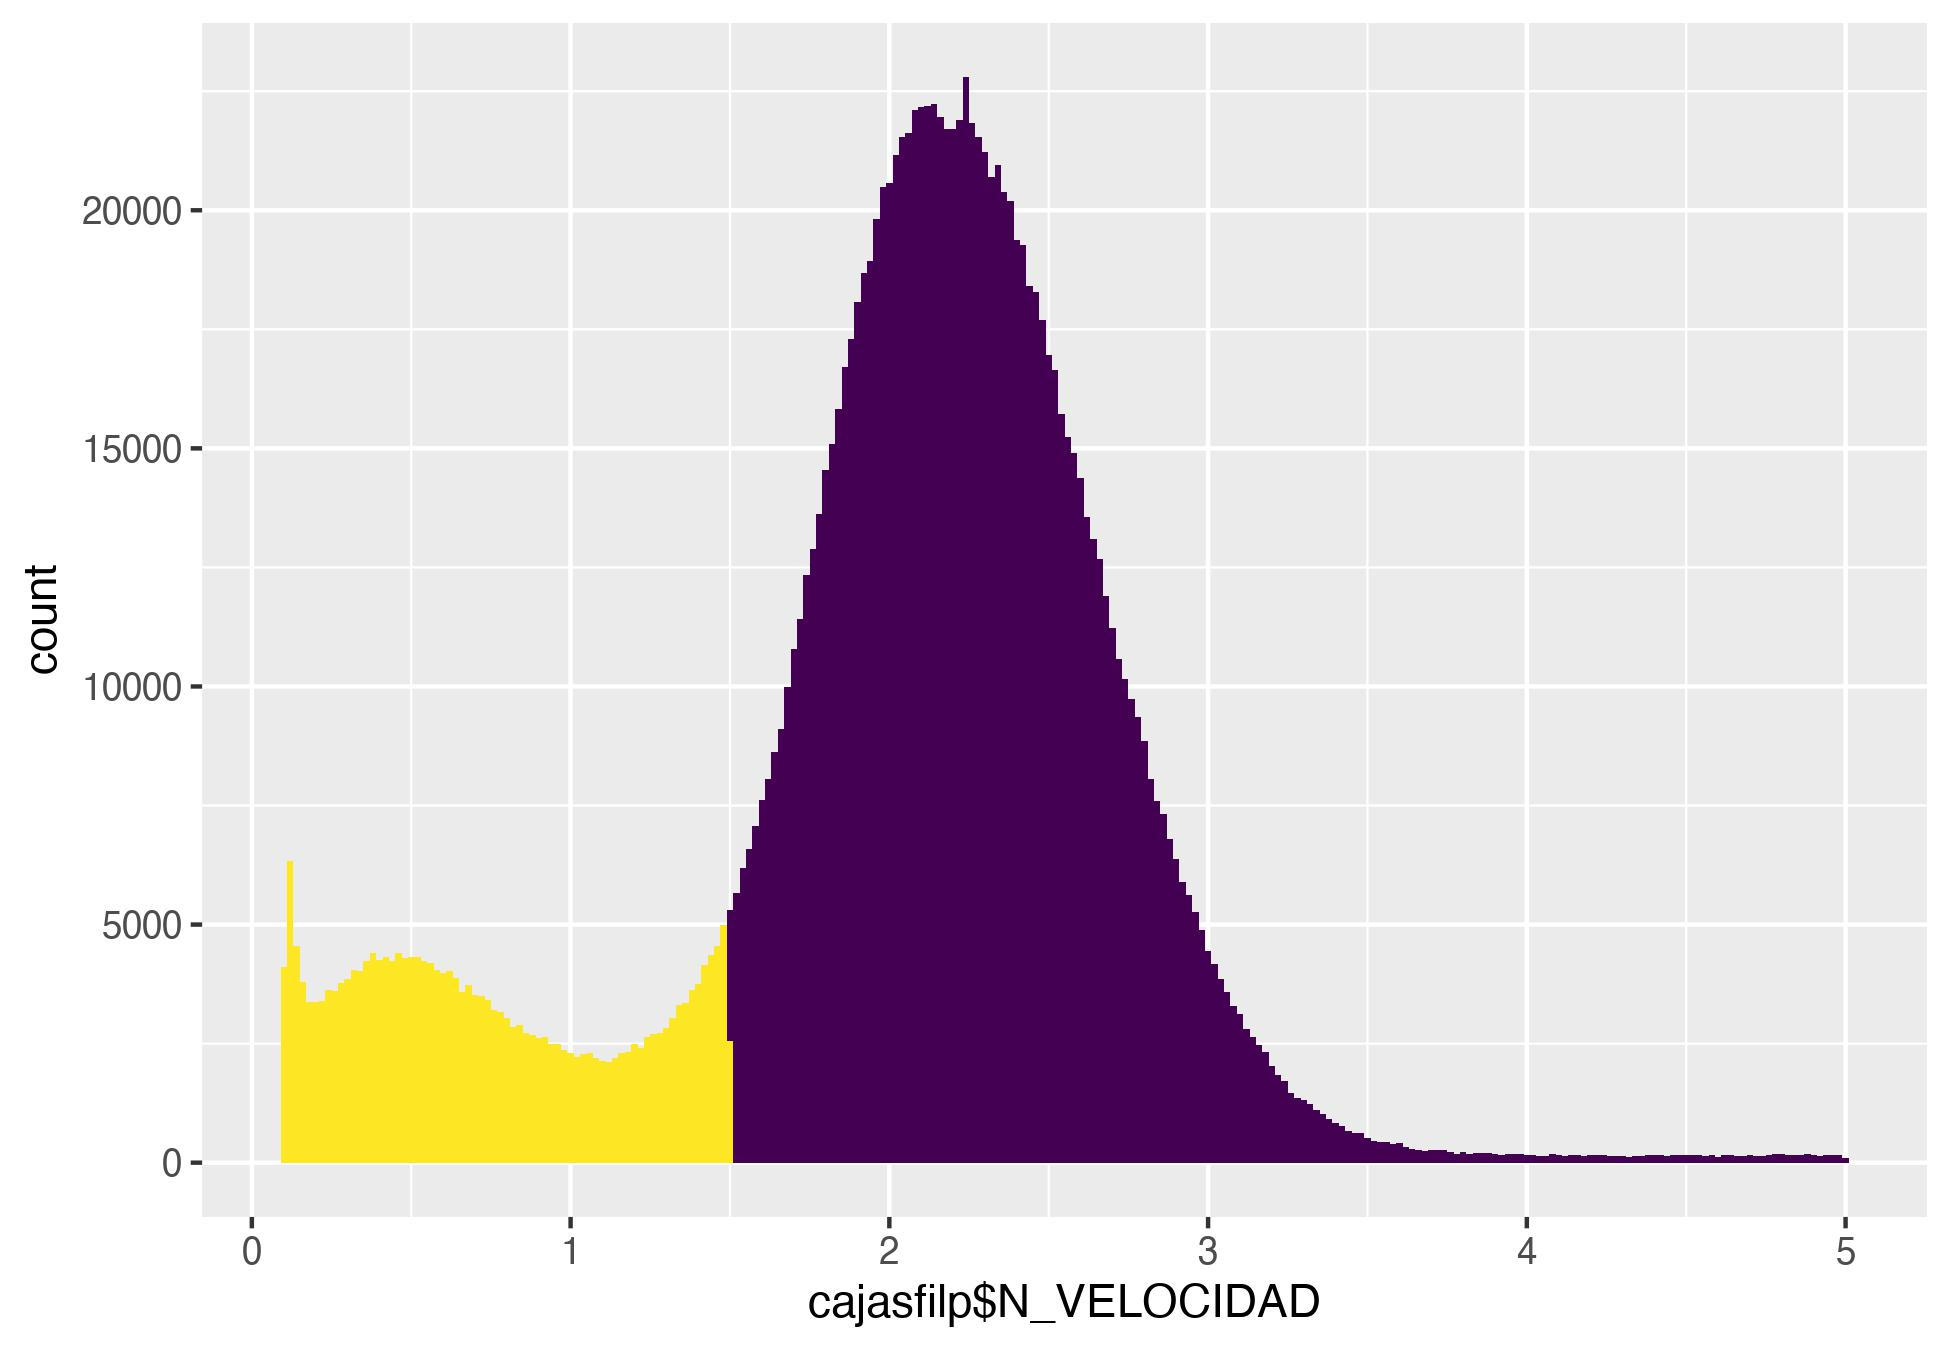
\includegraphics{SAR_Method_files/figure-latex/unnamed-chunk-20-1} \end{center}

3- Calcular el intervalo de tiempo entre registros sucesivos,

La idea es identificar los registros con tiempo efectivo de arrastre como lo muestra la Figura \ref{fig:esq};

\begin{figure}

{\centering \includegraphics[width=1\linewidth]{FIG/umbralveloc} 

}

\caption{\label{esq}Umbrarl de definiciones para calculo de velocidad de arrantre}\label{fig:esq}
\end{figure}

De esta forma, a cada señal proporcionada por la caja verde se le asignó una actividad: pesca, maniobra o navegada. En la figura 8 se puede ver un histograma que representa el número de registros en función de la velocidad para los registros filtrados, en él se observa cómo han desaparecido los registros en puerto y que existen tres modas correspondientes a las actividades mencionadas, maniobras (M), pesca (P) y navegaciones (N). (\protect\hyperlink{ref-Cohan2012}{Cojan, 2012})

Los registros en los cuales la velocidad del buque fue inferior a 1.5 nudos o entre 3.5 y 6 nudos, fueron considerados como maniobras de pesca (actividad ``M''), tales como la virada y largada del arte o el reposicionamiento del buque precedente al arrastre.

\begin{Shaded}
\begin{Highlighting}[]
\NormalTok{cajasfil2 }\OtherTok{\textless{}{-}}\NormalTok{ cajasfil }\SpecialCharTok{\%\textgreater{}\%}
  \FunctionTok{mutate}\NormalTok{(}\AttributeTok{MANIOBRA =} \FunctionTok{case\_when}\NormalTok{(}
\NormalTok{    N\_VELOCIDAD }\SpecialCharTok{\textgreater{}=} \DecValTok{0} \SpecialCharTok{\&}\NormalTok{ N\_VELOCIDAD }\SpecialCharTok{\textless{}} \FloatTok{1.5} \SpecialCharTok{\textasciitilde{}} \StringTok{"M"}\NormalTok{,}
\NormalTok{    N\_VELOCIDAD }\SpecialCharTok{\textgreater{}=} \FloatTok{1.5} \SpecialCharTok{\&}\NormalTok{ N\_VELOCIDAD }\SpecialCharTok{\textless{}} \FloatTok{3.5} \SpecialCharTok{\textasciitilde{}} \StringTok{"P"}\NormalTok{,}
\NormalTok{    N\_VELOCIDAD }\SpecialCharTok{\textgreater{}=} \FloatTok{3.5} \SpecialCharTok{\&}\NormalTok{ N\_VELOCIDAD }\SpecialCharTok{\textless{}} \DecValTok{6} \SpecialCharTok{\textasciitilde{}} \StringTok{"M"}\NormalTok{,}
\NormalTok{    N\_VELOCIDAD }\SpecialCharTok{\textgreater{}=} \DecValTok{6} \SpecialCharTok{\&}\NormalTok{ N\_VELOCIDAD }\SpecialCharTok{\textless{}=} \DecValTok{10} \SpecialCharTok{\textasciitilde{}} \StringTok{"N"}\NormalTok{,}
    \ConstantTok{TRUE} \SpecialCharTok{\textasciitilde{}} \ConstantTok{NA\_character\_}  \CommentTok{\# Por si acaso hay valores fuera de los rangos especificados}
\NormalTok{  ))}
\end{Highlighting}
\end{Shaded}

4- Diferenciar entre registros de pesca y no pesca basándose en la velocidad y solo dejó los registros \texttt{P}

\begin{Shaded}
\begin{Highlighting}[]
\NormalTok{cajasfilm }\OtherTok{\textless{}{-}}\NormalTok{ cajasfil2 }\SpecialCharTok{\%\textgreater{}\%} 
  \FunctionTok{filter}\NormalTok{(MANIOBRA}\SpecialCharTok{==}\StringTok{"P"}\NormalTok{)}
\end{Highlighting}
\end{Shaded}

5- Ahora calculo las distancias entre puntos. como??

\begin{Shaded}
\begin{Highlighting}[]
\CommentTok{\# Función para calcular la distancia entre dos puntos}
\NormalTok{calcular\_distancia }\OtherTok{\textless{}{-}} \ControlFlowTok{function}\NormalTok{(lat1, lon1, lat2, lon2) \{}
  \CommentTok{\# Convertir grados a radianes}
\NormalTok{  lat1\_rad }\OtherTok{\textless{}{-}}\NormalTok{ lat1 }\SpecialCharTok{*}\NormalTok{ pi }\SpecialCharTok{/} \DecValTok{180}
\NormalTok{  lon1\_rad }\OtherTok{\textless{}{-}}\NormalTok{ lon1 }\SpecialCharTok{*}\NormalTok{ pi }\SpecialCharTok{/} \DecValTok{180}
\NormalTok{  lat2\_rad }\OtherTok{\textless{}{-}}\NormalTok{ lat2 }\SpecialCharTok{*}\NormalTok{ pi }\SpecialCharTok{/} \DecValTok{180}
\NormalTok{  lon2\_rad }\OtherTok{\textless{}{-}}\NormalTok{ lon2 }\SpecialCharTok{*}\NormalTok{ pi }\SpecialCharTok{/} \DecValTok{180}
  
  \CommentTok{\# Radio de la Tierra en metros}
\NormalTok{  radio\_tierra }\OtherTok{\textless{}{-}} \DecValTok{6371000}
  
  \CommentTok{\# Calcular la distancia utilizando la fórmula del haversine}
\NormalTok{  dlat }\OtherTok{\textless{}{-}}\NormalTok{ lat2\_rad }\SpecialCharTok{{-}}\NormalTok{ lat1\_rad}
\NormalTok{  dlon }\OtherTok{\textless{}{-}}\NormalTok{ lon2\_rad }\SpecialCharTok{{-}}\NormalTok{ lon1\_rad}
\NormalTok{  a }\OtherTok{\textless{}{-}} \FunctionTok{sin}\NormalTok{(dlat }\SpecialCharTok{/} \DecValTok{2}\NormalTok{)}\SpecialCharTok{\^{}}\DecValTok{2} \SpecialCharTok{+} \FunctionTok{cos}\NormalTok{(lat1\_rad) }\SpecialCharTok{*} \FunctionTok{cos}\NormalTok{(lat2\_rad) }\SpecialCharTok{*} \FunctionTok{sin}\NormalTok{(dlon }\SpecialCharTok{/} \DecValTok{2}\NormalTok{)}\SpecialCharTok{\^{}}\DecValTok{2}
\NormalTok{  c }\OtherTok{\textless{}{-}} \DecValTok{2} \SpecialCharTok{*} \FunctionTok{atan2}\NormalTok{(}\FunctionTok{sqrt}\NormalTok{(a), }\FunctionTok{sqrt}\NormalTok{(}\DecValTok{1} \SpecialCharTok{{-}}\NormalTok{ a))}
\NormalTok{  distancia }\OtherTok{\textless{}{-}}\NormalTok{ radio\_tierra }\SpecialCharTok{*}\NormalTok{ c}
  
  \FunctionTok{return}\NormalTok{(distancia)}
\NormalTok{\}}

\NormalTok{datos }\OtherTok{\textless{}{-}}\NormalTok{ cajasfilm}
\CommentTok{\# Convertir la columna de fecha y hora a un objeto POSIXct con lubridate}
\NormalTok{datos}\SpecialCharTok{$}\NormalTok{fecha\_hora }\OtherTok{\textless{}{-}} \FunctionTok{ymd\_hms}\NormalTok{(}\FunctionTok{paste}\NormalTok{(datos}\SpecialCharTok{$}\NormalTok{FECHA, datos}\SpecialCharTok{$}\NormalTok{HORA))}

\CommentTok{\# Ordenar el dataframe por fecha y hora}
\NormalTok{datos }\OtherTok{\textless{}{-}}\NormalTok{ datos }\SpecialCharTok{\%\textgreater{}\%} 
  \FunctionTok{arrange}\NormalTok{(fecha\_hora)}
\CommentTok{\# Calcular la distancia para cada fila del dataframe}
\NormalTok{datos}\SpecialCharTok{$}\NormalTok{distancia }\OtherTok{\textless{}{-}} \FunctionTok{mapply}\NormalTok{(calcular\_distancia,}
\NormalTok{                          datos}\SpecialCharTok{$}\NormalTok{N\_LATITUD,}
\NormalTok{                          datos}\SpecialCharTok{$}\NormalTok{N\_LONGITUD,}
                          \FunctionTok{lag}\NormalTok{(datos}\SpecialCharTok{$}\NormalTok{N\_LATITUD),}
                          \FunctionTok{lag}\NormalTok{(datos}\SpecialCharTok{$}\NormalTok{N\_LONGITUD))}

\CommentTok{\# La primera fila tendrá NA ya que no hay punto anterior}
\NormalTok{datos}\SpecialCharTok{$}\NormalTok{distancia[}\DecValTok{1}\NormalTok{] }\OtherTok{\textless{}{-}} \ConstantTok{NA}
\end{Highlighting}
\end{Shaded}

ahora dejo valores de distancia menores a 1 km (preguntar). Luego calculo las variables de velocidad en metros/seg. y tiempo recorrido por la rastra. filtro por distancia \textless{} 1000

\begin{Shaded}
\begin{Highlighting}[]
\NormalTok{datosfil }\OtherTok{\textless{}{-}}\NormalTok{ datos }\SpecialCharTok{\%\textgreater{}\%} 
  \FunctionTok{filter}\NormalTok{(distancia }\SpecialCharTok{\textless{}} \DecValTok{1000}\NormalTok{) }\SpecialCharTok{\%\textgreater{}\%} 
  \FunctionTok{mutate}\NormalTok{(}\AttributeTok{VELONUE =}\NormalTok{ N\_VELOCIDAD}\SpecialCharTok{*}\FloatTok{0.51444}\NormalTok{, }\CommentTok{\# de nudos a mts/seg}
         \AttributeTok{TIEMPO =}\NormalTok{ (distancia }\SpecialCharTok{/}\NormalTok{ VELONUE) }\SpecialCharTok{/} \DecValTok{60}\NormalTok{,}
         \AttributeTok{AREA =}\NormalTok{ distancia}\SpecialCharTok{*}\DecValTok{5}\NormalTok{) }\CommentTok{\# como ejemplo 5 mt de aperttura de draga (corroborar)}
\end{Highlighting}
\end{Shaded}

Gafico el tiempo y velocidad promedio por barco

\begin{Shaded}
\begin{Highlighting}[]
\NormalTok{plottiem }\OtherTok{\textless{}{-}} \FunctionTok{ggplot}\NormalTok{(datosfil }\SpecialCharTok{\%\textgreater{}\%} 
               \FunctionTok{group\_by}\NormalTok{(MATRICULA))}\SpecialCharTok{+}
  \FunctionTok{geom\_boxplot}\NormalTok{(}\FunctionTok{aes}\NormalTok{(}\AttributeTok{x =} \FunctionTok{reorder}\NormalTok{(MATRICULA, TIEMPO), }
                   \AttributeTok{y =}\NormalTok{ TIEMPO),}
               \AttributeTok{outlier.color  =} \StringTok{"blue"}\NormalTok{)}\SpecialCharTok{+}
  \FunctionTok{geom\_hline}\NormalTok{(}\AttributeTok{yintercept =} \DecValTok{10}\NormalTok{, }
             \AttributeTok{col=}\StringTok{"red"}\NormalTok{)}\SpecialCharTok{+}
  \FunctionTok{theme\_few}\NormalTok{()}\SpecialCharTok{+}
  \FunctionTok{theme}\NormalTok{(}\AttributeTok{axis.text.x =} \FunctionTok{element\_text}\NormalTok{(}\AttributeTok{angle =} \DecValTok{90}\NormalTok{,}
                                     \AttributeTok{hjust =} \DecValTok{1}\NormalTok{,}
                                     \AttributeTok{vjust =} \FloatTok{0.5}\NormalTok{,}
                                     \AttributeTok{size =} \DecValTok{5}\NormalTok{))}\SpecialCharTok{+}
  \FunctionTok{xlab}\NormalTok{(}\StringTok{"Matriculas"}\NormalTok{) }\SpecialCharTok{+}
  \FunctionTok{ylab}\NormalTok{(}\FunctionTok{expression}\NormalTok{(}\FunctionTok{paste}\NormalTok{(}\FunctionTok{Tiempo}\NormalTok{ (min))))}

\NormalTok{plotvel }\OtherTok{\textless{}{-}} \FunctionTok{ggplot}\NormalTok{(datosfil }\SpecialCharTok{\%\textgreater{}\%} 
               \FunctionTok{group\_by}\NormalTok{(MATRICULA))}\SpecialCharTok{+}
  \FunctionTok{geom\_boxplot}\NormalTok{(}\FunctionTok{aes}\NormalTok{(}\AttributeTok{x =} \FunctionTok{reorder}\NormalTok{(MATRICULA, VELONUE),}
                   \AttributeTok{y =}\NormalTok{ VELONUE),}
               \AttributeTok{outlier.color  =} \StringTok{"red"}\NormalTok{)}\SpecialCharTok{+}
  \FunctionTok{theme\_few}\NormalTok{()}\SpecialCharTok{+}
  \FunctionTok{theme}\NormalTok{(}\AttributeTok{axis.text.x =} \FunctionTok{element\_text}\NormalTok{(}\AttributeTok{angle =} \DecValTok{90}\NormalTok{,}
                                     \AttributeTok{hjust =} \DecValTok{1}\NormalTok{,}
                                     \AttributeTok{vjust =} \FloatTok{0.5}\NormalTok{,}
                                     \AttributeTok{size =} \DecValTok{5}\NormalTok{))}\SpecialCharTok{+}
  \FunctionTok{xlab}\NormalTok{(}\StringTok{"Matriculas"}\NormalTok{) }\SpecialCharTok{+}
  \FunctionTok{ylab}\NormalTok{(}\FunctionTok{expression}\NormalTok{(}\FunctionTok{paste}\NormalTok{(}\FunctionTok{Velocidad}\NormalTok{ (m}\SpecialCharTok{/}\NormalTok{s))))}
  
  \CommentTok{\#facet\_wrap(.\textasciitilde{}MES)}
\FunctionTok{ggarrange}\NormalTok{(plottiem, plotvel, }\AttributeTok{ncol =} \DecValTok{1}\NormalTok{)}
\end{Highlighting}
\end{Shaded}

\begin{center}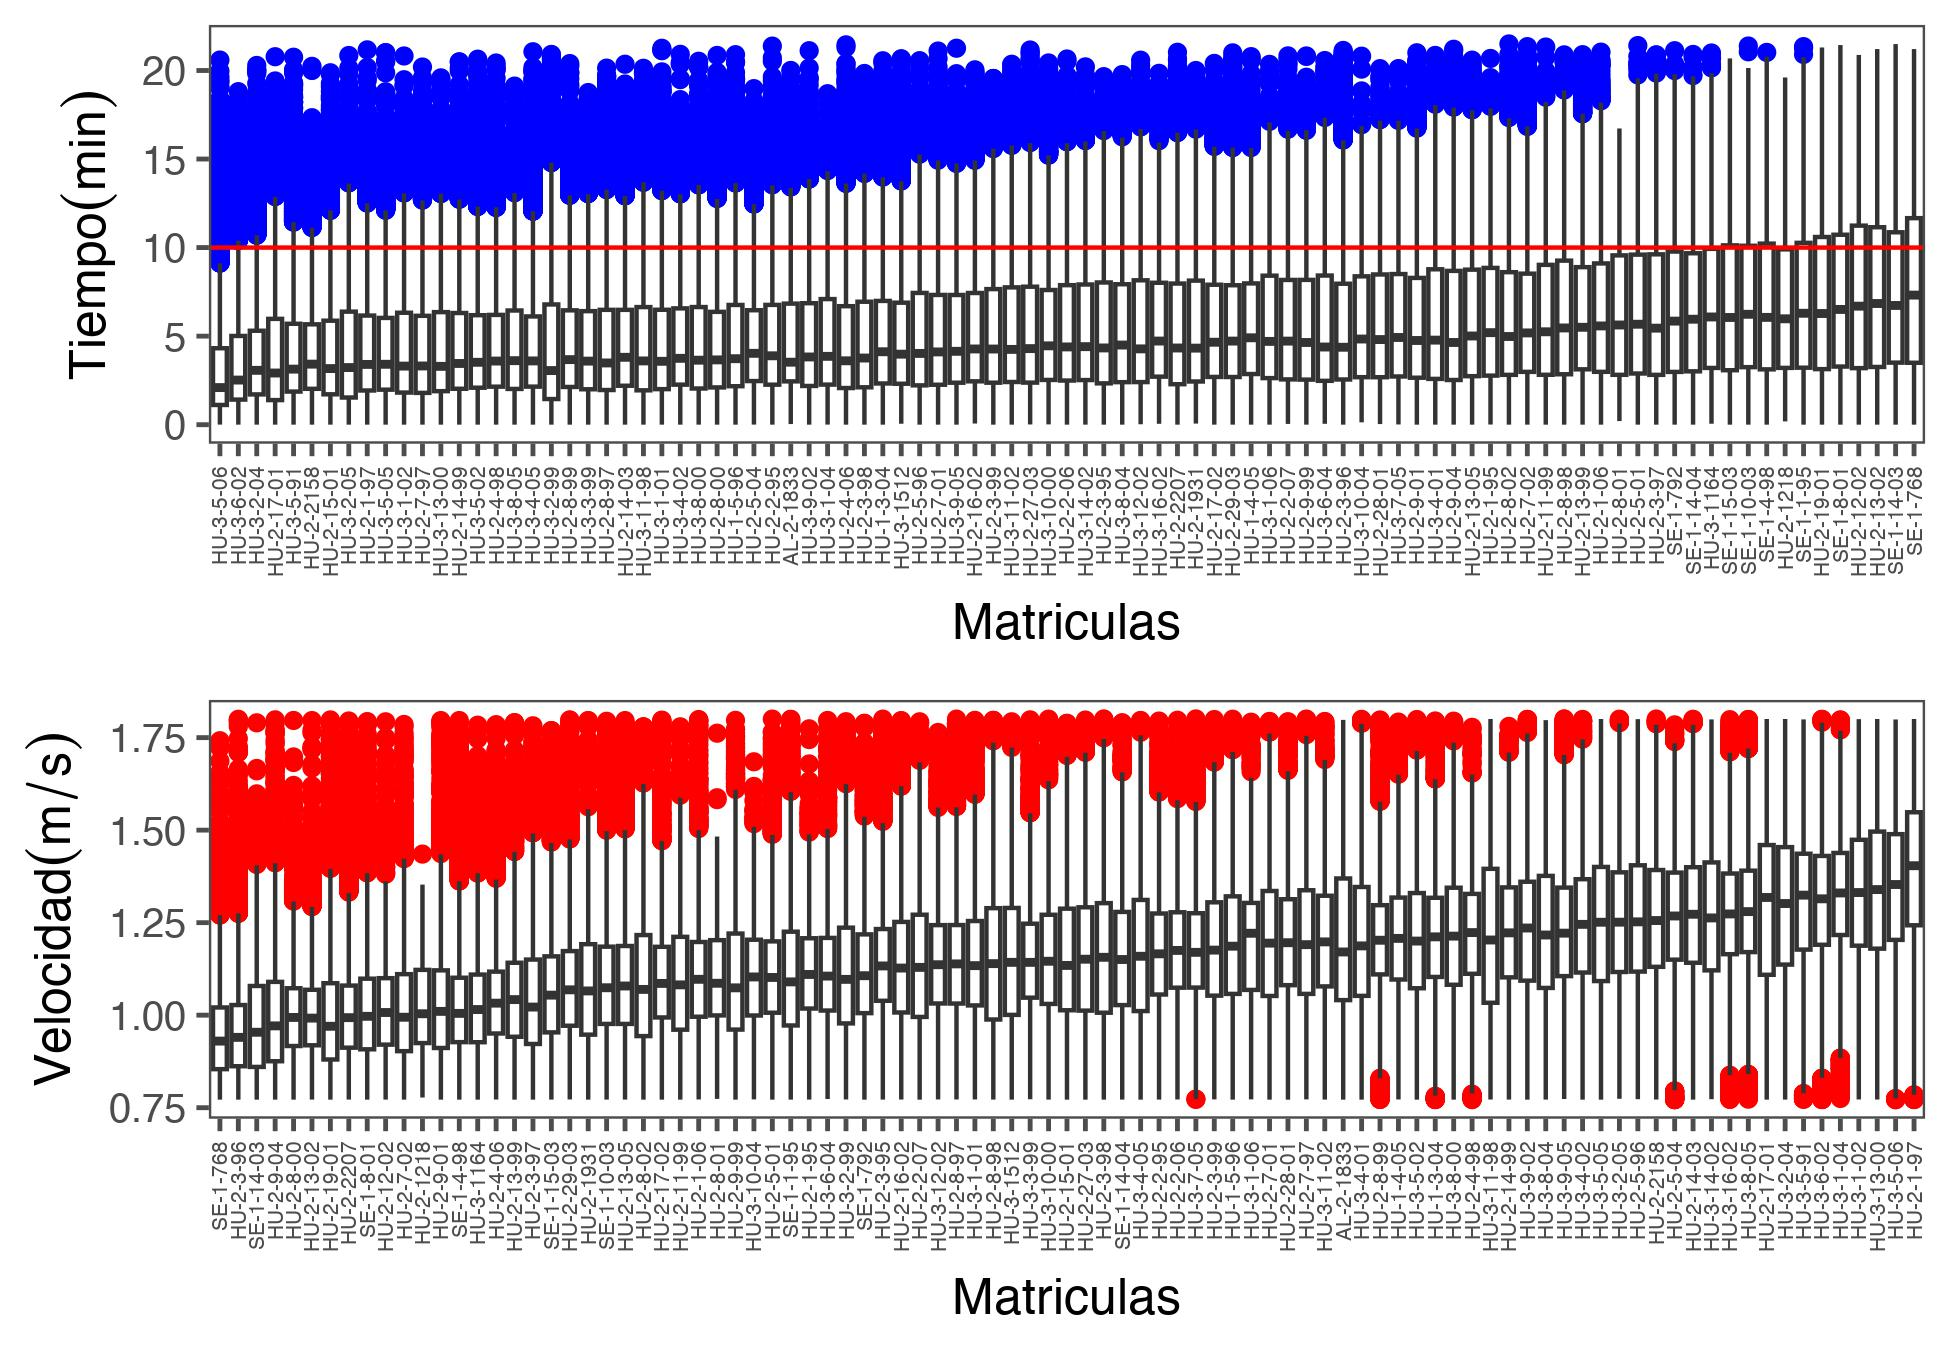
\includegraphics{SAR_Method_files/figure-latex/unnamed-chunk-25-1} \end{center}

Calculo el SAR

De acuerdo a Church et al. (\protect\hyperlink{ref-Church2016}{2016}), el Cálculo de la Proporción del Área Barrida (Swept Area Ratio, SAR) SA es el área barrida (mts/2), CA es el área de la celda y SAR es la proporción del área barrida (equivalente al número de veces que la celda fue barrida).

donde;

\[
SAr = \frac{SA}{CA}
\]

donde \texttt{SA}sera la distancia recorrida el arrastre y la apertura en metros del draga, es decir;

\[
SA = Distancia \times Apertura de draga
\]

Ahora se debe proceder a egrillar este dato en las celdas

\hypertarget{mapas}{%
\section{MAPAS}\label{mapas}}

Ahora produzco un mapa de las grillas utilizadas en la pesquería de Chirla. Estos datos vectoriales fueron obtenidos desde la paina oficial de datos espaciales de la Junta de Andalucia \href{https://portalrediam.cica.es/descargas?path=\%2F08_AMBITOS_INTERES_AMBIENTAL\%2F02_LITORAL_MARINO\%2F04_SOCIOECONOMIA\%2FZonasProduccionMoluscos}{Shapesfile}

\hypertarget{leo-shapes-y-transformo-a-la-proyecciuxf3n-correcta.}{%
\subsection{Leo Shapes y transformo a la proyección correcta.}\label{leo-shapes-y-transformo-a-la-proyecciuxf3n-correcta.}}

\begin{verbatim}
## Reading layer `costa_proyectada' from data source 
##   `/Users/mauriciomardones/IEO/IN_BENTOS/SHP_Chirla/costa_proyectada.shp' 
##   using driver `ESRI Shapefile'
## Simple feature collection with 10 features and 4 fields
## Geometry type: POLYGON
## Dimension:     XY
## Bounding box:  xmin: -34115.27 ymin: 3891271 xmax: 301588.8 ymax: 4173659
## Projected CRS: WGS_1984_Complex_UTM_Zone_30N
\end{verbatim}

\begin{verbatim}
## Reading layer `cuadriculas_definitivo' from data source 
##   `/Users/mauriciomardones/IEO/IN_BENTOS/SHP_Chirla/cuadriculas_definitivo.shp' 
##   using driver `ESRI Shapefile'
## Simple feature collection with 219 features and 2 fields
## Geometry type: POLYGON
## Dimension:     XY
## Bounding box:  xmin: 109273.6 ymin: 4071852 xmax: 198073.5 ymax: 4125446
## Projected CRS: ETRS89 / UTM zone 30N
\end{verbatim}

\begin{verbatim}
## Reading layer `batimetria_rediam20x20_10m_id' from data source 
##   `/Users/mauriciomardones/IEO/IN_BENTOS/SHP_Chirla/batimetria_rediam20x20_10m_id.shp' 
##   using driver `ESRI Shapefile'
## Simple feature collection with 1 feature and 1 field
## Geometry type: MULTIPOLYGON
## Dimension:     XY
## Bounding box:  xmin: 99337.29 ymin: 4070000 xmax: 201873.6 ymax: 4127412
## Projected CRS: ETRS89 / UTM zone 30N
\end{verbatim}

\hypertarget{transforma-data}{%
\subsection{Transforma data}\label{transforma-data}}

\begin{Shaded}
\begin{Highlighting}[]
\NormalTok{grilla1 }\OtherTok{\textless{}{-}} \FunctionTok{st\_transform}\NormalTok{(grilla, }
                        \StringTok{"+init=epsg:4326"}\NormalTok{)}
\NormalTok{costandalucia1 }\OtherTok{\textless{}{-}} \FunctionTok{st\_transform}\NormalTok{(costandalucia,}
                               \StringTok{"+init=epsg:4326"}\NormalTok{)}
\NormalTok{bati1 }\OtherTok{\textless{}{-}} \FunctionTok{st\_transform}\NormalTok{(bati,}
                      \StringTok{"+init=epsg:4326"}\NormalTok{)}
\end{Highlighting}
\end{Shaded}

\hypertarget{mapa}{%
\section{Mapa}\label{mapa}}

\begin{Shaded}
\begin{Highlighting}[]
\NormalTok{mas }\OtherTok{\textless{}{-}} \FunctionTok{ggplot}\NormalTok{() }\SpecialCharTok{+}
  \CommentTok{\#geom\_sf(data = lito1, fill="white", color="blue") +}
  \FunctionTok{geom\_sf}\NormalTok{(}\AttributeTok{data =}\NormalTok{ grilla1, }\AttributeTok{fill=}\StringTok{"white"}\NormalTok{, }\AttributeTok{color=}\StringTok{"red"}\NormalTok{) }\SpecialCharTok{+}
  \FunctionTok{geom\_sf}\NormalTok{(}\AttributeTok{data =}\NormalTok{ costandalucia1, }\AttributeTok{fill=}\StringTok{"\#fee8c8"}\NormalTok{) }\SpecialCharTok{+}
  \CommentTok{\#geom\_sf(data = bati1, fill="white", color="blue") +}
  \CommentTok{\# geom\_sf(data = fisicomar1, alpha=0.1,}
  \CommentTok{\#         linetype=5) +}
  \FunctionTok{scale\_fill\_viridis\_d}\NormalTok{(}\AttributeTok{option=}\StringTok{"H"}\NormalTok{,}
                       \AttributeTok{alpha=}\NormalTok{.}\DecValTok{5}\NormalTok{)}\SpecialCharTok{+}
  \FunctionTok{coord\_sf}\NormalTok{() }\SpecialCharTok{+}
  \FunctionTok{xlab}\NormalTok{(}\FunctionTok{expression}\NormalTok{(}\FunctionTok{paste}\NormalTok{(Longitude}\SpecialCharTok{\^{}}\NormalTok{o,}\SpecialCharTok{\textasciitilde{}}\StringTok{\textquotesingle{}O\textquotesingle{}}\NormalTok{))) }\SpecialCharTok{+}
  \FunctionTok{ylab}\NormalTok{(}\FunctionTok{expression}\NormalTok{(}\FunctionTok{paste}\NormalTok{(Latitude}\SpecialCharTok{\^{}}\NormalTok{o,}\SpecialCharTok{\textasciitilde{}}\StringTok{\textquotesingle{}S\textquotesingle{}}\NormalTok{)))}\SpecialCharTok{+}
  \CommentTok{\# ggrepel::geom\_label\_repel(}
  \CommentTok{\#   data = zonapro1,}
  \CommentTok{\#   aes(label = ZONA, geometry = geometry),}
  \CommentTok{\#   stat = "sf\_coordinates",}
  \CommentTok{\#   min.segment.length = ,}
  \CommentTok{\#   colour = "black",}
  \CommentTok{\#   size = 2,}
  \CommentTok{\#   segment.colour = "black",}
  \CommentTok{\#   box.padding = 0.7,}
  \CommentTok{\#   max.overlaps = 50) +}
  \FunctionTok{theme\_few}\NormalTok{()}\SpecialCharTok{+}
  \FunctionTok{theme}\NormalTok{(}\AttributeTok{legend.position =} \StringTok{"none"}\NormalTok{)}\SpecialCharTok{+}
  \FunctionTok{xlim}\NormalTok{(}\SpecialCharTok{{-}}\FloatTok{7.6}\NormalTok{,}\SpecialCharTok{{-}}\DecValTok{6}\NormalTok{)}\SpecialCharTok{+}
  \FunctionTok{ylim}\NormalTok{(}\FloatTok{36.6}\NormalTok{, }\FloatTok{37.4}\NormalTok{)}
\NormalTok{mas}
\end{Highlighting}
\end{Shaded}

\begin{center}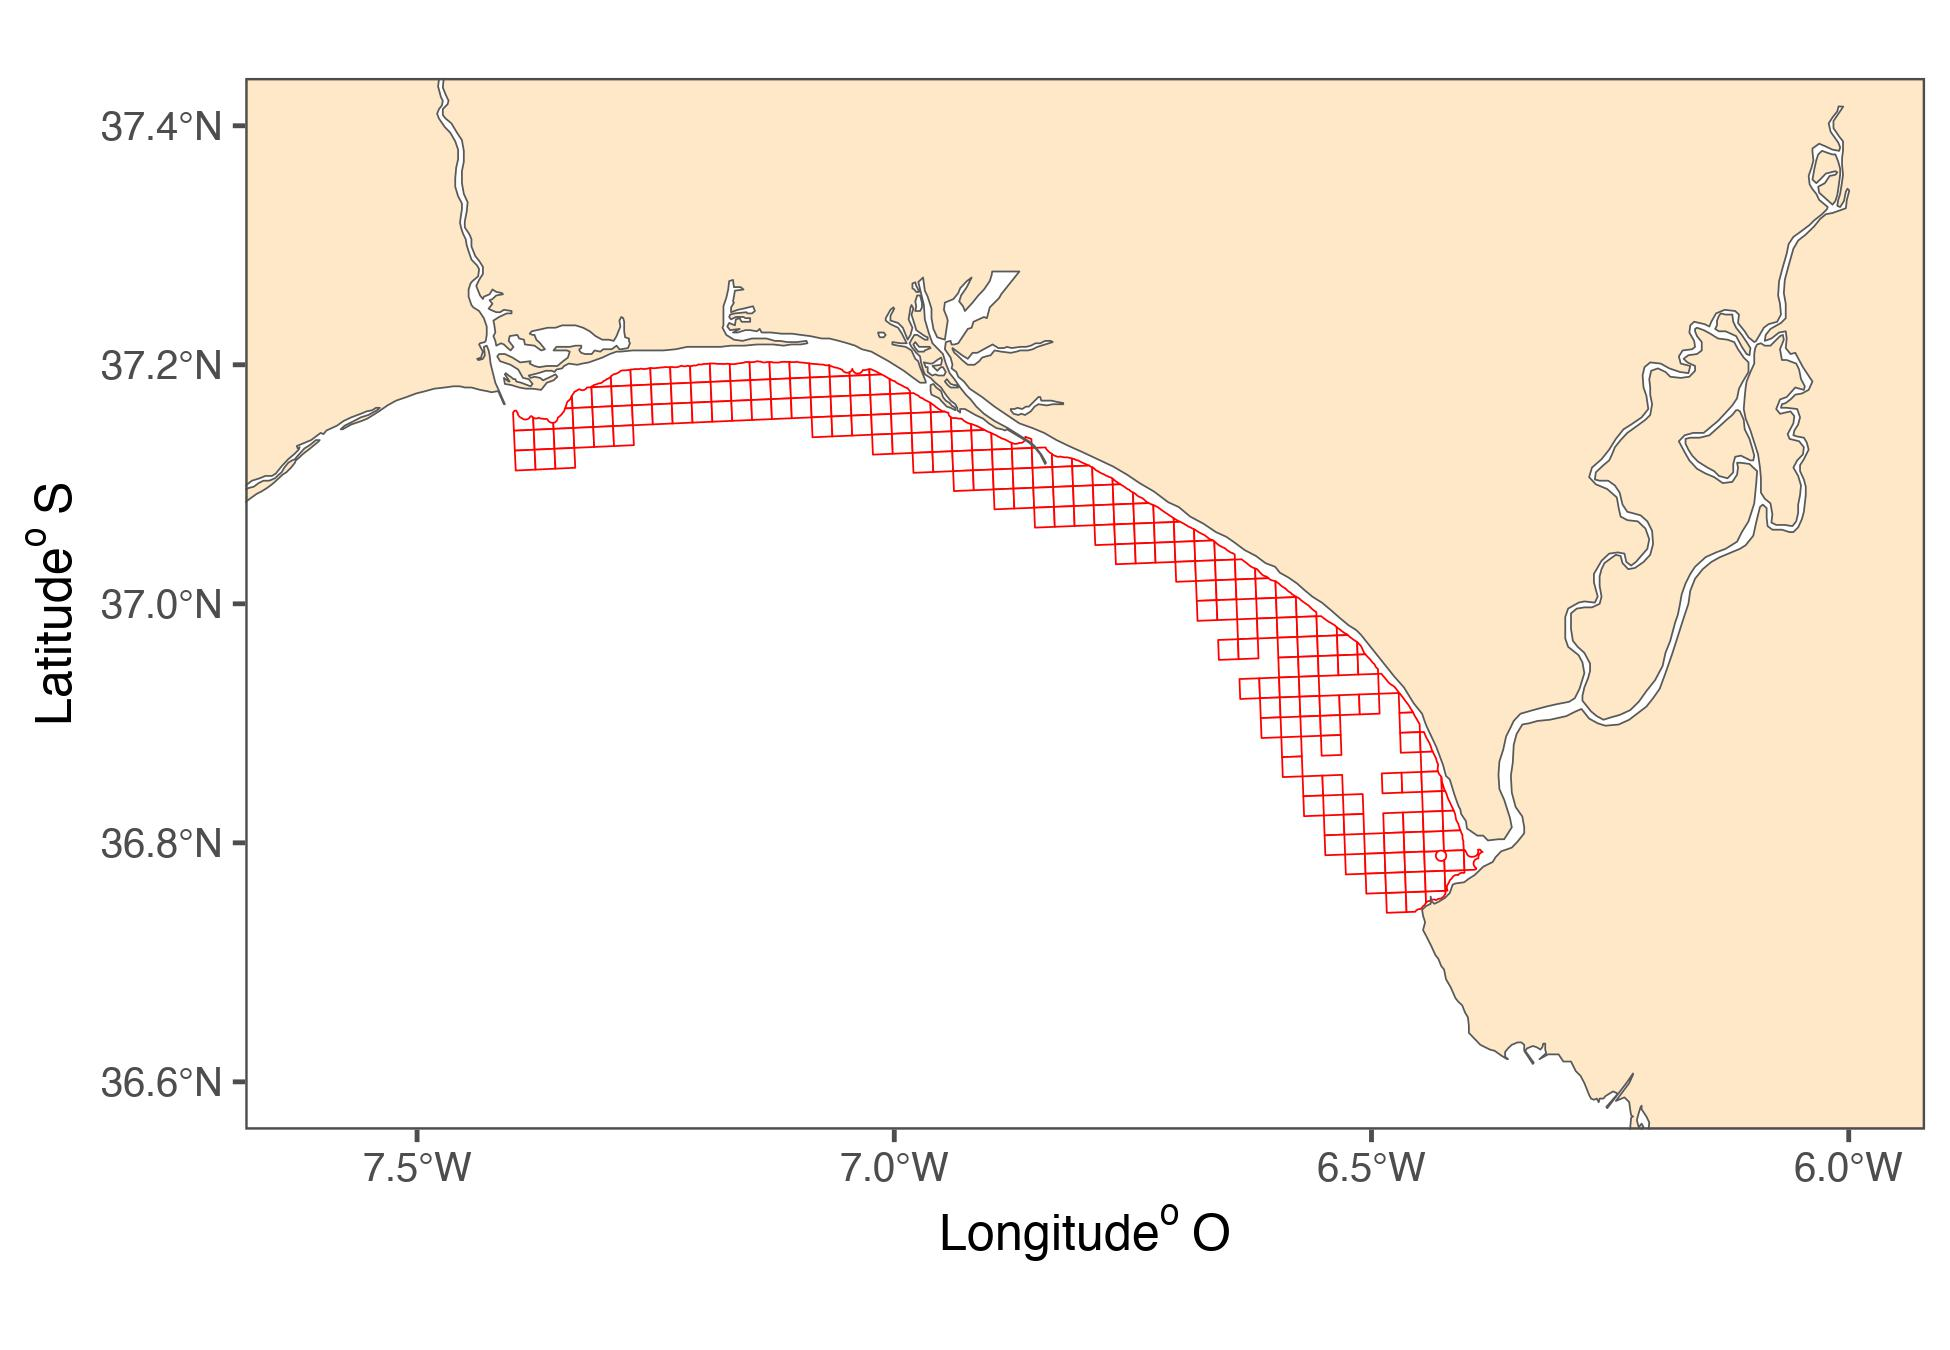
\includegraphics{SAR_Method_files/figure-latex/unnamed-chunk-28-1} \end{center}

Ahora identifico la base que quiero plotear

\begin{Shaded}
\begin{Highlighting}[]
\FunctionTok{names}\NormalTok{(rendi)}
\end{Highlighting}
\end{Shaded}

\begin{verbatim}
##  [1] "Estaciones"              "Observaciones"          
##  [3] "Date"                    "Track"                  
##  [5] "Track (m)"               "depth_i"                
##  [7] "depth_f"                 "depth_m"                
##  [9] "vel_i"                   "vel_f"                  
## [11] "vel_m"                   "hora_i"                 
## [13] "hora_f"                  "g...14"                 
## [15] "min...15"                "g...16"                 
## [17] "min...17"                "LAT"                    
## [19] "LONG"                    "Nºrejillas"             
## [21] "Vol (l.)...21"           "Vol (l.)...22"          
## [23] "P (total + cascajo) (g)" "SW_tolva"               
## [25] "CSW"                     "CSW_tolva"              
## [27] "N"                       "N_tolva"                
## [29] "area"                    "dens"                   
## [31] "bio"                     "P cascajo (g)"          
## [33] "P cascajo_tolva"         "Tow_time"               
## [35] "PComercial (kg)"         "rend"                   
## [37] "ID"                      "FP"
\end{verbatim}

\begin{Shaded}
\begin{Highlighting}[]
\NormalTok{rendi2 }\OtherTok{\textless{}{-}}\NormalTok{ rendi }\SpecialCharTok{\%\textgreater{}\%} 
  \FunctionTok{mutate}\NormalTok{(}\AttributeTok{LONG1 =}\NormalTok{ LONG}\SpecialCharTok{*{-}}\DecValTok{1}\NormalTok{) }\SpecialCharTok{\%\textgreater{}\%} 
  \FunctionTok{st\_as\_sf}\NormalTok{(}\AttributeTok{coords =} \FunctionTok{c}\NormalTok{(}\StringTok{"LONG1"}\NormalTok{, }\StringTok{"LAT"}\NormalTok{),  }
                  \AttributeTok{crs =} \StringTok{"+init=epsg:4326"}\NormalTok{) }
\end{Highlighting}
\end{Shaded}

This grid has the same characteristics as the environmental data grids
that will be called up later. This grid is 1x0.5 degrees which allows a
clear visualization of the processes, whether biological and/or
environmental.

\begin{Shaded}
\begin{Highlighting}[]
\CommentTok{\#Aca dejo este code para hacer una grilla}
\CommentTok{\# Grid\textless{}{-} suba1aa  \%\textgreater{}\% \#pm481 es el plot base original linea 481}
\CommentTok{\#   sf::st\_make\_grid(cellsize = c(1,0.5)) \%\textgreater{}\% \# para que quede cuadrada}
\CommentTok{\#   sf::st\_cast("MULTIPOLYGON") \%\textgreater{}\%}
\CommentTok{\#   sf::st\_sf()  \%\textgreater{}\%  \# objeto en spatial feature}
\CommentTok{\#   dplyr::mutate(cellid = row\_number()) }
\CommentTok{\# }
\CommentTok{\# \# Clean the input data by removing duplicate vertices and making the object topologically valid}
\CommentTok{\# grid3 \textless{}{-} st\_make\_valid(Grid)}
\CommentTok{\# }
\CommentTok{\# \# Corto la grilla dentro de las SSMU}
\CommentTok{\# \#gridcrop1 \textless{}{-} crop\_shape(grid3, suba1aa, polygon = TRUE)}

\CommentTok{\# the first object drives the output geometry}
\NormalTok{grilla2 }\OtherTok{\textless{}{-}}\NormalTok{ grilla1 }\SpecialCharTok{\%\textgreater{}\%}
  \FunctionTok{rename}\NormalTok{(}\StringTok{"Estaciones"} \OtherTok{=} \StringTok{"ID\_CELDA"}\NormalTok{) }
\CommentTok{\# ahora uno}
\NormalTok{grilla3 }\OtherTok{\textless{}{-}} \FunctionTok{st\_join}\NormalTok{(grilla2, rendi2)}
\FunctionTok{names}\NormalTok{(grilla3)}
\end{Highlighting}
\end{Shaded}

\begin{verbatim}
##  [1] "Estaciones.x"            "area.x"                 
##  [3] "Estaciones.y"            "Observaciones"          
##  [5] "Date"                    "Track"                  
##  [7] "Track (m)"               "depth_i"                
##  [9] "depth_f"                 "depth_m"                
## [11] "vel_i"                   "vel_f"                  
## [13] "vel_m"                   "hora_i"                 
## [15] "hora_f"                  "g...14"                 
## [17] "min...15"                "g...16"                 
## [19] "min...17"                "LONG"                   
## [21] "Nºrejillas"              "Vol (l.)...21"          
## [23] "Vol (l.)...22"           "P (total + cascajo) (g)"
## [25] "SW_tolva"                "CSW"                    
## [27] "CSW_tolva"               "N"                      
## [29] "N_tolva"                 "area.y"                 
## [31] "dens"                    "bio"                    
## [33] "P cascajo (g)"           "P cascajo_tolva"        
## [35] "Tow_time"                "PComercial (kg)"        
## [37] "rend"                    "ID"                     
## [39] "FP"                      "geometry"
\end{verbatim}

repito el mapa con rendimientos

\begin{Shaded}
\begin{Highlighting}[]
\NormalTok{masrend }\OtherTok{\textless{}{-}} \FunctionTok{ggplot}\NormalTok{() }\SpecialCharTok{+}
  \CommentTok{\#geom\_sf(data = lito1, fill="white", color="blue") +}
  \CommentTok{\#geom\_sf(data = grilla1, fill="white", color="red") +}
  \FunctionTok{geom\_sf}\NormalTok{(}\AttributeTok{data =}\NormalTok{ costandalucia1, }\AttributeTok{fill=}\StringTok{"\#fee8c8"}\NormalTok{) }\SpecialCharTok{+}
  \FunctionTok{geom\_sf}\NormalTok{(}\AttributeTok{data =}\NormalTok{ grilla3 }\SpecialCharTok{\%\textgreater{}\%} 
          \FunctionTok{drop\_na}\NormalTok{(rend), }
          \FunctionTok{aes}\NormalTok{(}\AttributeTok{fill=}\FunctionTok{cut}\NormalTok{(rend,}
                       \AttributeTok{breaks =} \FunctionTok{seq}\NormalTok{(}\DecValTok{0}\NormalTok{, }\DecValTok{20}\NormalTok{, }\AttributeTok{by =} \DecValTok{2}\NormalTok{))))}\SpecialCharTok{+}
  \CommentTok{\# geom\_sf(data = fisicomar1, alpha=0.1,}
  \CommentTok{\#         linetype=5) +}
  \FunctionTok{scale\_fill\_brewer}\NormalTok{(}\AttributeTok{type =} \StringTok{"qual"}\NormalTok{,}
                    \CommentTok{\#labels = label, \# if you must}
                    \AttributeTok{palette =} \StringTok{"BrBG,"}\NormalTok{,}
                    \AttributeTok{name =} \StringTok{"CPUE"}\NormalTok{) }\SpecialCharTok{+}
    \FunctionTok{coord\_sf}\NormalTok{() }\SpecialCharTok{+}
  \FunctionTok{xlab}\NormalTok{(}\FunctionTok{expression}\NormalTok{(}\FunctionTok{paste}\NormalTok{(Longitude}\SpecialCharTok{\^{}}\NormalTok{o,}\SpecialCharTok{\textasciitilde{}}\StringTok{\textquotesingle{}O\textquotesingle{}}\NormalTok{))) }\SpecialCharTok{+}
  \FunctionTok{ylab}\NormalTok{(}\FunctionTok{expression}\NormalTok{(}\FunctionTok{paste}\NormalTok{(Latitude}\SpecialCharTok{\^{}}\NormalTok{o,}\SpecialCharTok{\textasciitilde{}}\StringTok{\textquotesingle{}S\textquotesingle{}}\NormalTok{)))}\SpecialCharTok{+}
  \CommentTok{\# ggrepel::geom\_label\_repel(}
  \CommentTok{\#   data = zonapro1,}
  \CommentTok{\#   aes(label = ZONA, geometry = geometry),}
  \CommentTok{\#   stat = "sf\_coordinates",}
  \CommentTok{\#   min.segment.length = ,}
  \CommentTok{\#   colour = "black",}
  \CommentTok{\#   size = 2,}
  \CommentTok{\#   segment.colour = "black",}
  \CommentTok{\#   box.padding = 0.7,}
  \CommentTok{\#   max.overlaps = 50) +}
  \FunctionTok{theme\_few}\NormalTok{()}\SpecialCharTok{+}
  \FunctionTok{theme}\NormalTok{(}\AttributeTok{legend.position =} \StringTok{"bottom"}\NormalTok{)}\SpecialCharTok{+}
  \FunctionTok{xlim}\NormalTok{(}\SpecialCharTok{{-}}\FloatTok{7.6}\NormalTok{,}\SpecialCharTok{{-}}\DecValTok{6}\NormalTok{)}\SpecialCharTok{+}
  \FunctionTok{ylim}\NormalTok{(}\FloatTok{36.6}\NormalTok{, }\FloatTok{37.4}\NormalTok{)}

\NormalTok{masrend}
\end{Highlighting}
\end{Shaded}

\begin{center}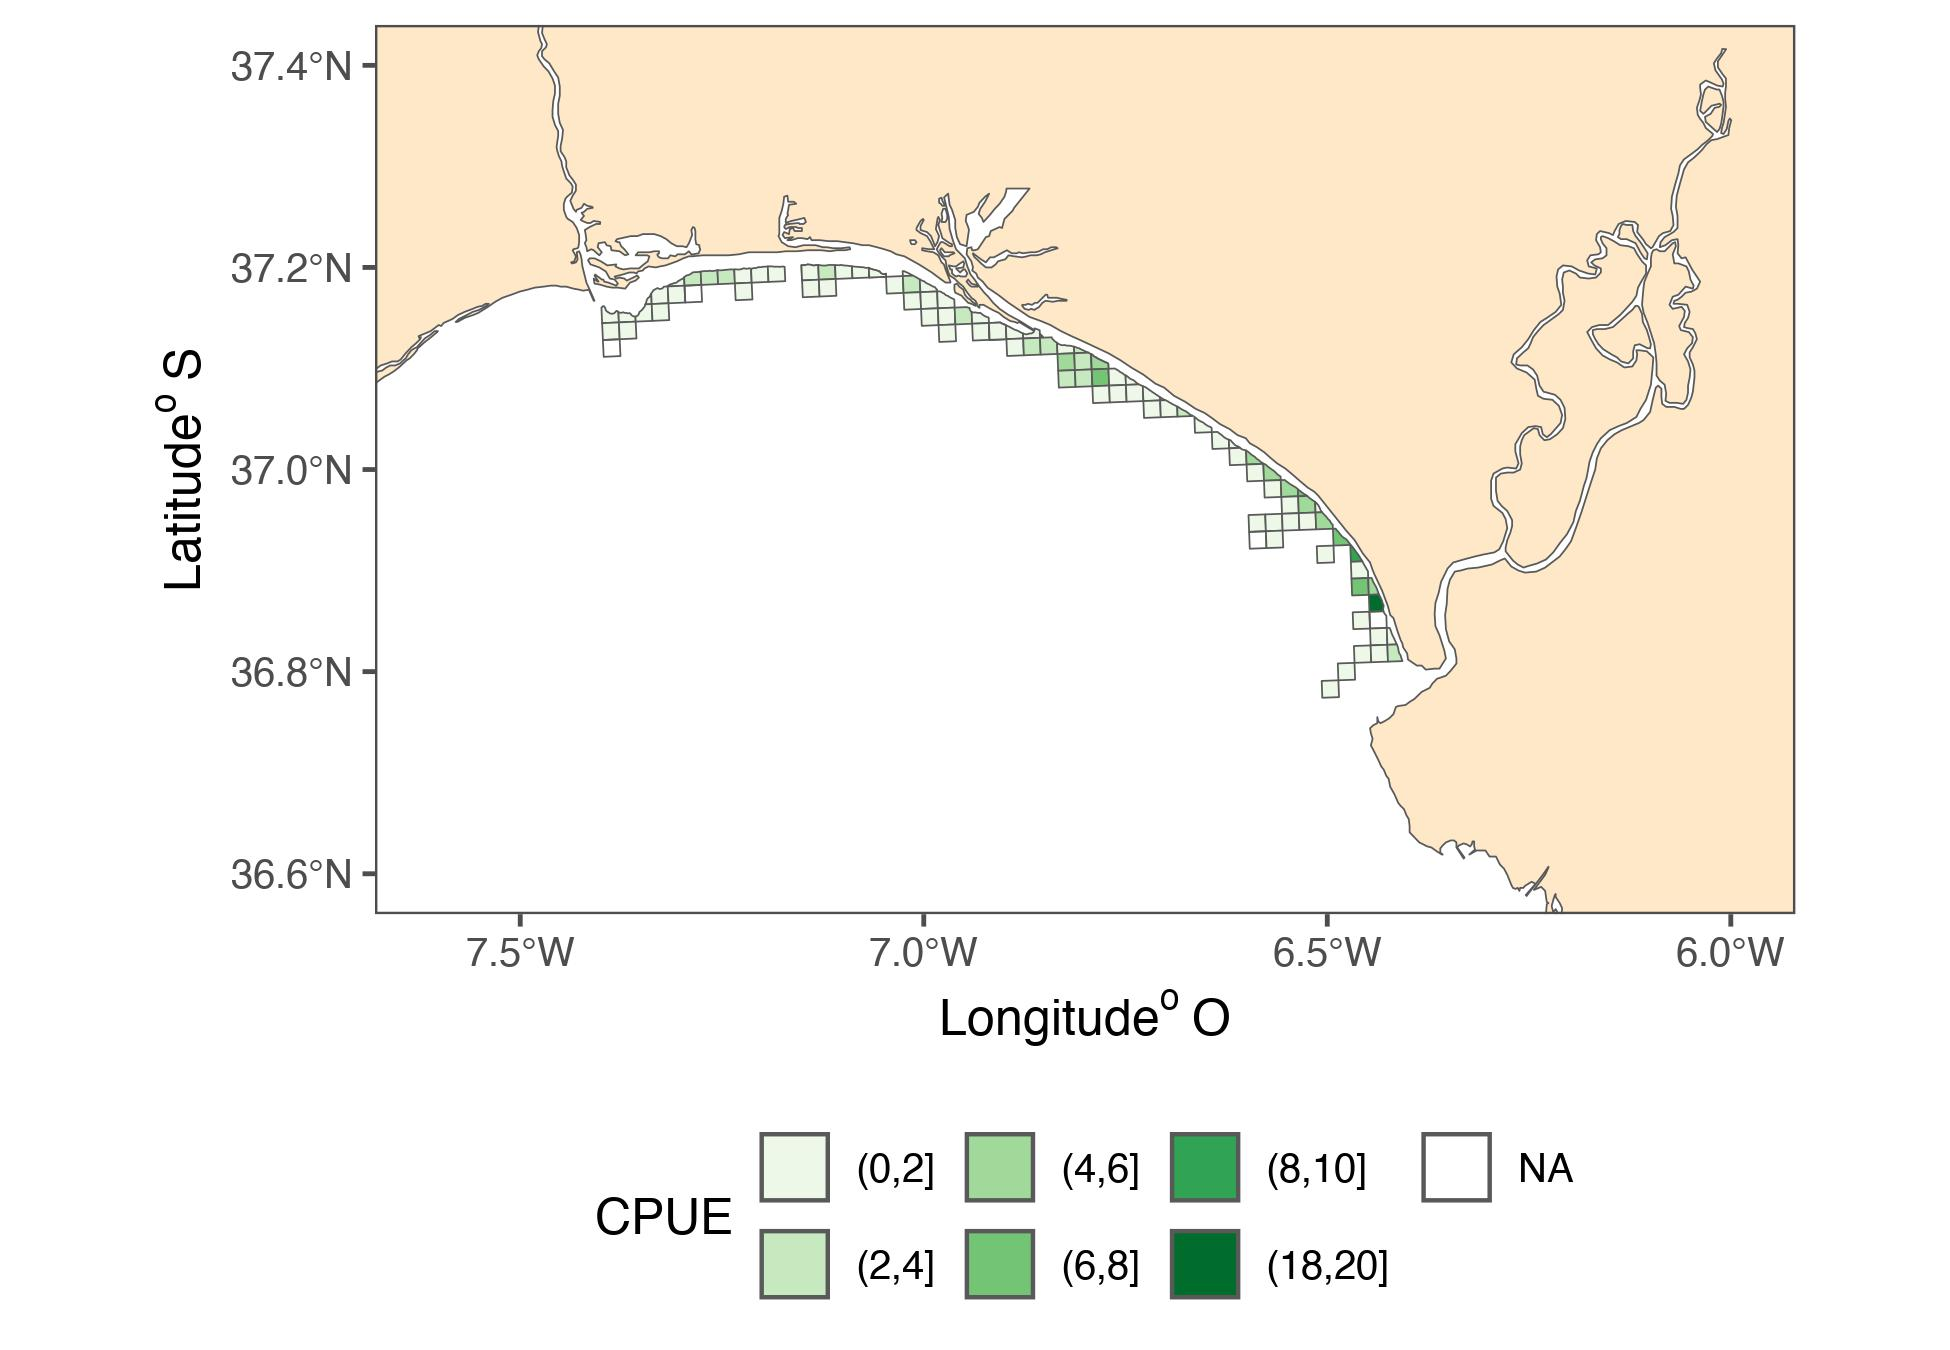
\includegraphics{SAR_Method_files/figure-latex/unnamed-chunk-29-1} \end{center}

repito el mapa con rendimientos

\begin{Shaded}
\begin{Highlighting}[]
\NormalTok{mascapt }\OtherTok{\textless{}{-}} \FunctionTok{ggplot}\NormalTok{() }\SpecialCharTok{+}
  \CommentTok{\#geom\_sf(data = lito1, fill="white", color="blue") +}
  \CommentTok{\#geom\_sf(data = grilla1, fill="white", color="red") +}
  \FunctionTok{geom\_sf}\NormalTok{(}\AttributeTok{data =}\NormalTok{ costandalucia1, }\AttributeTok{fill=}\StringTok{"\#fee8c8"}\NormalTok{) }\SpecialCharTok{+}
  \FunctionTok{geom\_sf}\NormalTok{(}\AttributeTok{data =}\NormalTok{ grilla3 }\SpecialCharTok{\%\textgreater{}\%}
            \FunctionTok{drop\_na}\NormalTok{(}\StringTok{\textasciigrave{}}\AttributeTok{PComercial (kg)}\StringTok{\textasciigrave{}}\NormalTok{) }\SpecialCharTok{\%\textgreater{}\%} 
            \FunctionTok{filter}\NormalTok{(}\StringTok{\textasciigrave{}}\AttributeTok{PComercial (kg)}\StringTok{\textasciigrave{}}\SpecialCharTok{\textgreater{}}\FloatTok{0.01}\NormalTok{), }
          \FunctionTok{aes}\NormalTok{(}\AttributeTok{fill=}\FunctionTok{cut}\NormalTok{(}\StringTok{\textasciigrave{}}\AttributeTok{PComercial (kg)}\StringTok{\textasciigrave{}}\NormalTok{,}
                       \AttributeTok{breaks =} \FunctionTok{seq}\NormalTok{(}\DecValTok{0}\NormalTok{, }\DecValTok{50}\NormalTok{, }\AttributeTok{by =} \DecValTok{5}\NormalTok{))))}\SpecialCharTok{+}
  \CommentTok{\# geom\_sf(data = fisicomar1, alpha=0.1,}
  \CommentTok{\#         linetype=5) +}
  \FunctionTok{scale\_fill\_brewer}\NormalTok{(}\AttributeTok{type =} \StringTok{"qual"}\NormalTok{,}
                    \CommentTok{\#labels = label, \# if you must}
                    \AttributeTok{palette =} \StringTok{"GnBu"}\NormalTok{,}
                    \AttributeTok{name =} \StringTok{"Capturas"}\NormalTok{) }\SpecialCharTok{+}
    \FunctionTok{coord\_sf}\NormalTok{() }\SpecialCharTok{+}
  \FunctionTok{xlab}\NormalTok{(}\FunctionTok{expression}\NormalTok{(}\FunctionTok{paste}\NormalTok{(Longitude}\SpecialCharTok{\^{}}\NormalTok{o,}\SpecialCharTok{\textasciitilde{}}\StringTok{\textquotesingle{}O\textquotesingle{}}\NormalTok{))) }\SpecialCharTok{+}
  \FunctionTok{ylab}\NormalTok{(}\FunctionTok{expression}\NormalTok{(}\FunctionTok{paste}\NormalTok{(Latitude}\SpecialCharTok{\^{}}\NormalTok{o,}\SpecialCharTok{\textasciitilde{}}\StringTok{\textquotesingle{}S\textquotesingle{}}\NormalTok{)))}\SpecialCharTok{+}
  \CommentTok{\# ggrepel::geom\_label\_repel(}
  \CommentTok{\#   data = zonapro1,}
  \CommentTok{\#   aes(label = ZONA, geometry = geometry),}
  \CommentTok{\#   stat = "sf\_coordinates",}
  \CommentTok{\#   min.segment.length = ,}
  \CommentTok{\#   colour = "black",}
  \CommentTok{\#   size = 2,}
  \CommentTok{\#   segment.colour = "black",}
  \CommentTok{\#   box.padding = 0.7,}
  \CommentTok{\#   max.overlaps = 50) +}
  \FunctionTok{theme\_few}\NormalTok{()}\SpecialCharTok{+}
  \FunctionTok{theme}\NormalTok{(}\AttributeTok{legend.position =} \StringTok{"bottom"}\NormalTok{)}\SpecialCharTok{+}
  \FunctionTok{xlim}\NormalTok{(}\SpecialCharTok{{-}}\FloatTok{7.6}\NormalTok{,}\SpecialCharTok{{-}}\DecValTok{6}\NormalTok{)}\SpecialCharTok{+}
  \FunctionTok{ylim}\NormalTok{(}\FloatTok{36.6}\NormalTok{, }\FloatTok{37.4}\NormalTok{)}

\NormalTok{mascapt}
\end{Highlighting}
\end{Shaded}

\begin{center}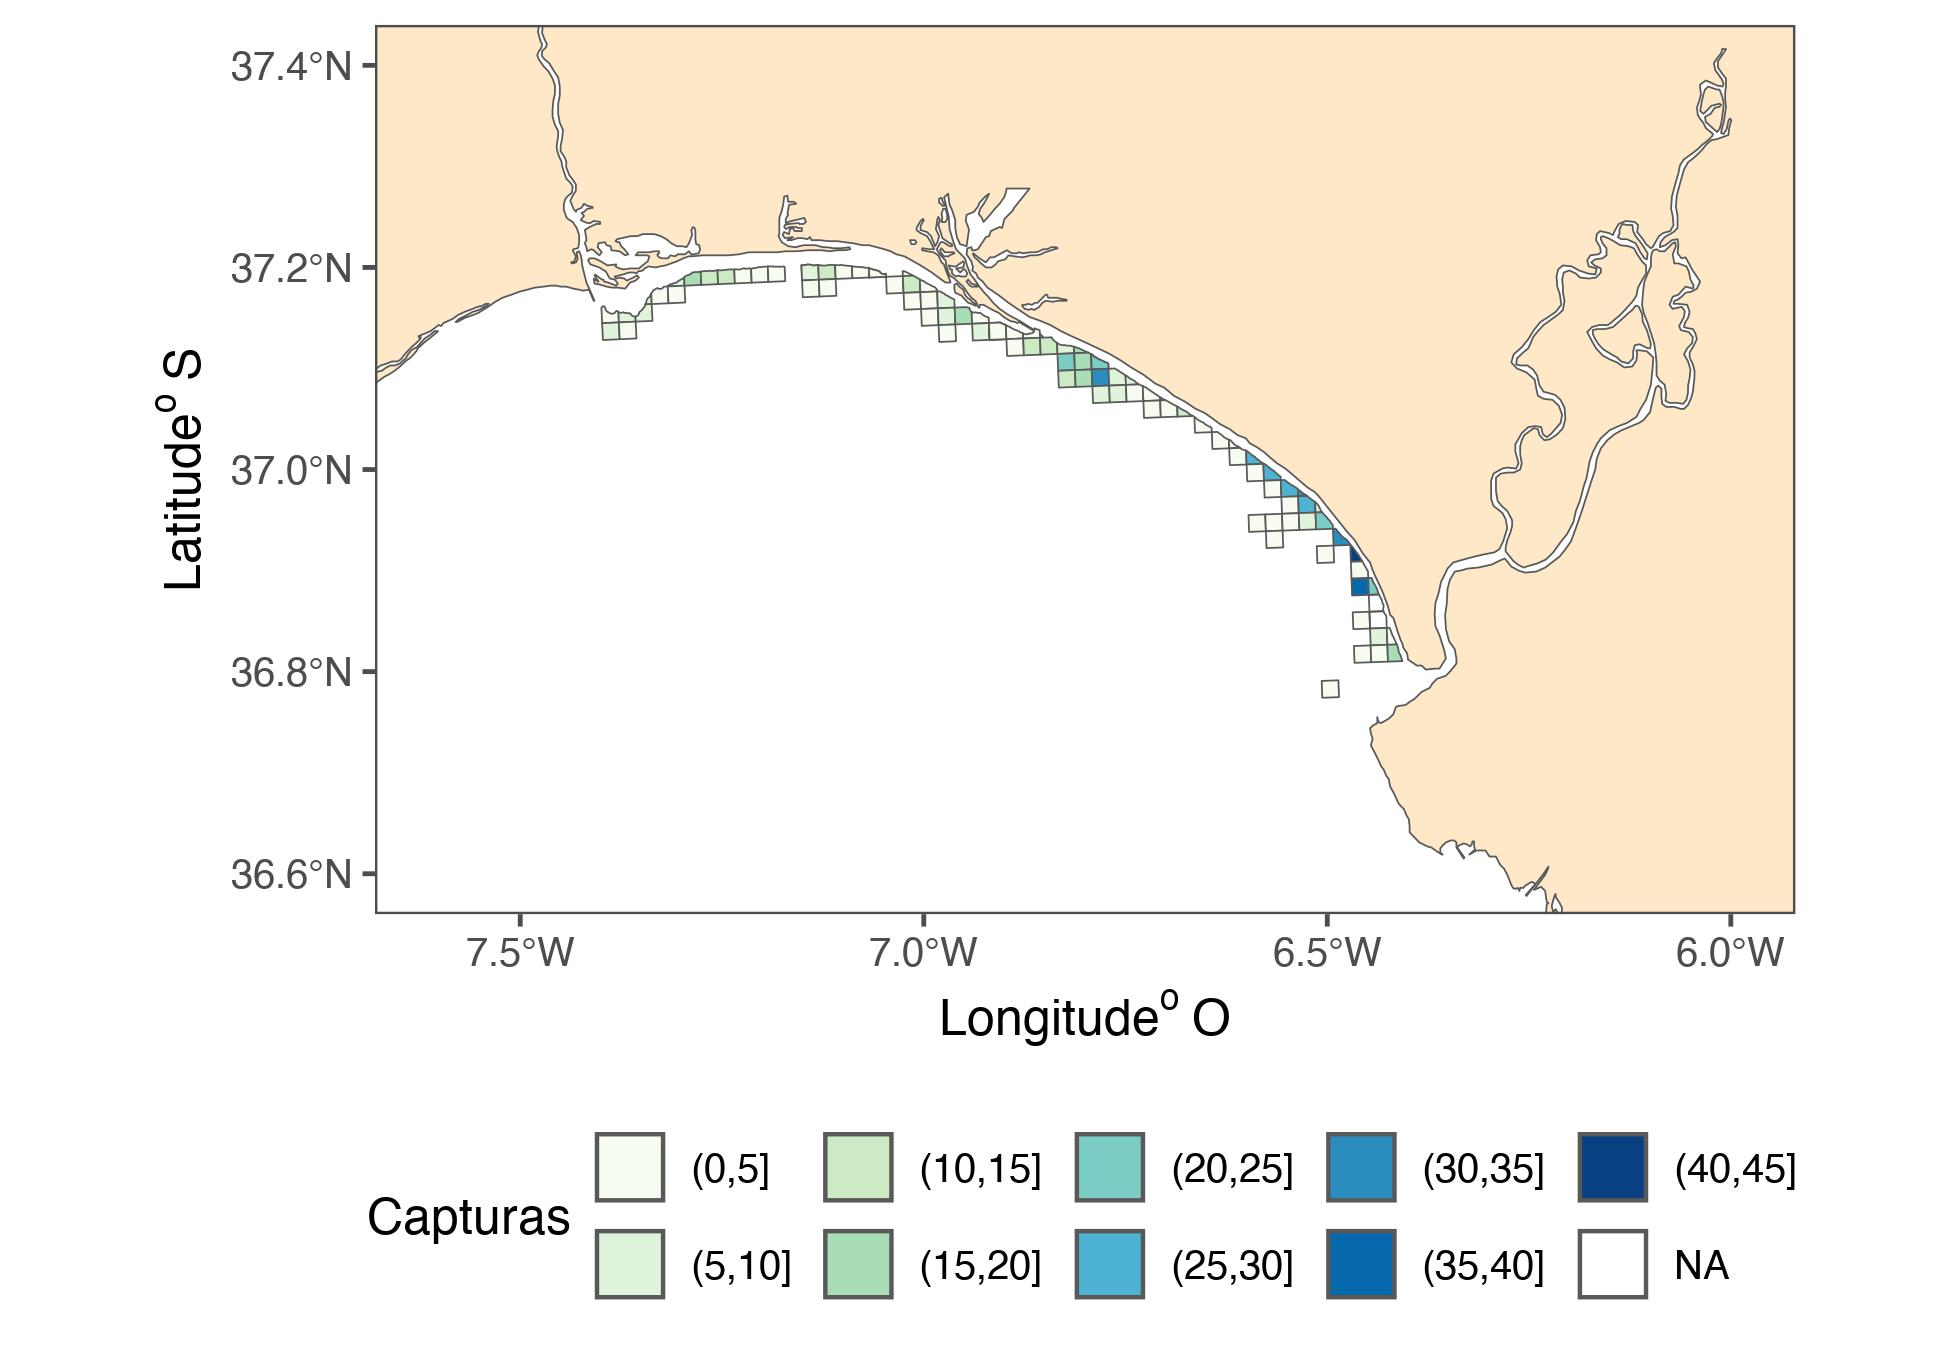
\includegraphics{SAR_Method_files/figure-latex/unnamed-chunk-30-1} \end{center}

\newpage

\hypertarget{referencias}{%
\section*{REFERENCIAS}\label{referencias}}
\addcontentsline{toc}{section}{REFERENCIAS}

\hypertarget{refs}{}
\begin{CSLReferences}{1}{0}
\leavevmode\vadjust pre{\hypertarget{ref-Church2016}{}}%
Church, N. J., Carter, A. J., Tobin, D., Edwards, D., Eassom, A., Cameron, A., Johnson, G. E., Robson, L. M., \& Webb, K. E. (2016). {JNCC Pressure Mapping Methodology. Physical Damage (Reversible Change)-Penetration and/or disturbance of the substrate below the surface of the seabed, including abrasion}. \emph{JNCC Report No}, \emph{515}(December).

\leavevmode\vadjust pre{\hypertarget{ref-Cohan2012}{}}%
Cojan, M. (2012). \emph{{AN{Á}LISIS Y SEGUIMIENTO DE LA FLOTA DE DRAGAS HIDR{Á}ULICAS EN EL GOLFO DE C{Á}DIZ}} (pp. 1--23) {[}PhD thesis{]}.

\leavevmode\vadjust pre{\hypertarget{ref-Indicator}{}}%
Indicator, C. (n.d.). \emph{{CEMP GUIDELINES FOR Common indicator Sentinels of the Seabed ( SoS )}} (pp. 1--38).

\end{CSLReferences}

\end{document}
